\documentclass[10pt,a4paper]{article}
\usepackage{ngerman}
\usepackage[utf8]{inputenc}
\usepackage{sectsty, xcolor}
\usepackage{lastpage}
\usepackage{amsmath, amsfonts, amssymb, enumitem, fancyhdr, graphicx, float, makeidx, textcomp, multicol}
\usepackage[hidelinks]{hyperref}
\usepackage[hang,flushmargin]{footmisc}
\usepackage{listings}
\lstloadlanguages{HTML}
\definecolor{pblue}{rgb}{0.13,0.13,1}
\definecolor{pgreen}{rgb}{0,0.5,0}
\definecolor{pred}{rgb}{0.9,0,0}
\definecolor{pgrey}{rgb}{0.46,0.45,0.48}
\definecolor{background}{rgb}{0.95,0.95,0.92}
\lstset{language=HTML,
  backgroundcolor=\color{background},
  frame=single,
  rulecolor=\color{pgrey},
  showspaces=false,
  showtabs=false,
  breaklines=true,
  showstringspaces=false,
  breakatwhitespace=true,
  commentstyle=\color{pgreen},
  keywordstyle=\color{pblue},
  stringstyle=\color{pred},
  breaklines=true,
  numbers=left,
  numberstyle=\tiny\color{pgrey},
  basicstyle=\ttfamily\footnotesize,
  inputencoding=utf8,
  extendedchars=true,
  literate={ä}{{\"a}}1 {ö}{{\"o}}1 {ü}{{\"u}}1,
  moredelim=[il][\textcolor{pgrey}]{\$\$},
  moredelim=[is][\textcolor{pgrey}]{\%\%}{\%\%}
}
\makeindex

\definecolor{dunkelblau}{rgb}{0,0.4,0.6}
\subsectionfont{\color{dunkelblau}}

\title{WEBT FS 2020}
\author{Victor Fernández}
\date{Februar 2020}

\addtolength{\oddsidemargin}{-.875in}
\addtolength{\evensidemargin}{-.875in}
\addtolength{\textwidth}{1.75in}
\addtolength{\topmargin}{-.875in}
\addtolength{\textheight}{1.75in}

% muss nach Änderung der margin kommen!
\pagestyle{fancy}
\fancyhf{} %reset
\fancyhead[L]{HSLU}
\fancyhead[C]{WEBT}
\fancyhead[R]{\thepage/\pageref{LastPage}}
\fancyfoot[L]{}
\fancyfoot[C]{}
\fancyfoot[R]{}
\renewcommand{\headrulewidth}{0.2pt} % Strich in Kopfzeile

\begin{document}

\maketitle
\tableofcontents
\thispagestyle{empty}
\pagebreak

\part{SW 01 - Networking Today \& Networking Trends}
\section{Lernziele (Leitfragen)}
\begin{enumerate}
    \item Wieso sind Computernetzwerke wichtig in unserem Leben?
    \item Wieso sind Computernetzwerke wichtig für Unternehmen und unsere Berufe?
    \item Wieso ist Kenntnis der Computernetzwerke wichtig für die Wirtschaftsinformatik?
    \item Was ist ein \flqq End Device\frqq{} (Endgerät)? Geben Sie Beispiele.
    \item Was ist ein ``intermediary (network) device'' (Netzwerkkomponente), oder Netzwerkgerät? Geben Sie Beispiele.
    \item Wie funktioniert das \flqq Client-Server\frqq{} Modell? Geben Sie Beispiele.
    \item Wie funktioniert das \flqq Peer-to-peer\frqq{} Modell? Geben Sie Beispiele.
    \item Wie unterscheiden sich physikalische und logische Netzwerkdiagramme?
    \item Wie kann man anhand ihrer Grösse Computernetzwerke klassifizieren?
    \item Wie unterschieden sich LANs und WANs? Was ist ihre Beziehung?
    \item Was ist das Internet? Wer besitzt das Internet? Was für Organisationen sind in der Entwicklung des Internets beteiligt?
    \item Was ist der Unterschied zwischen einem Intranet und einem Extranet?
    \item Wie verbinden sich normalerweise Häuser, Wohnungen und HomeOffices mit dem Internet?
    \item Wie verbinden sich normalerweise Büros und Unternehmern mit dem Internet?
    \item Was bedeutet Konvergenz im Kontext der Computernetzwerke?
    \item Was bedeutet \flqq fault tolerance\frqq{}  (Fehlertoleranz) im Kontext der Computernetzwerke? Geben Sie ein Beispiel
    \item Was bedeutet \flqq scalability\frqq{}  (Skalierbarkeit) im Kontext der Computernetzwerke? Geben Sie ein Beispiel
    \item Was bedeutet \flqq quality of service (QoS)\frqq{}  im Kontext der Computernetzwerke? Geben Sie ein Beispiel
    \item Wieso ist Netzwerksicherheit wichtig?
    \item Was sind die drei Hauptinformationssicherheitsziele?
    \item Was ist \flqq BYOD\frqq{}  und was sind seine Auswirkungen für Geschäfte und Unternehmen?
    \item Was ist \flqq cloud computing\frqq{} ? Was für Cloud Arten gibt es?
    \item Was ist die Verbindung zwischen \flqq cloud computing\frqq{}  und Computernetzwerken?
\end{enumerate}

\section{Antworten}
\subsection*{Wieso sind Computernetzwerke wichtig in unserem Leben?}
Die zunehmende Digitalisierung erfordert eine immer grössere Vernetzung im Alltag. Sei es beruflich mit E-Mails, Website, Dateitransfer, cloudbasierte Lösungen etc. oder auch privat mit digitalem Fernsehen, Streamingangeboten von Videos und Musik, bis zur Smart-Watch.
\subsection*{Wieso sind Computernetzwerke wichtig für Unternehmen und unsere Berufe?}
Für moderne Unternehmen ist es heutzutage wichtig vernetzt zu sein. Man verfügt beispielsweise über IP-Telefone, Fileserver, Mailserver, Virtual-Machine-Server, Rendering-Server etc. Um auf all diese Dienste zugreifen zu können, muss ein Computernetzwerk bestehen.
\subsection*{Wieso ist Kenntnis der Computernetzwerke wichtig für die Wirtschaftsinformatik?}
Die Berufsausrichtung/-aussicht der Wirtschaftsinformatikspezialisten tendiert dazu, dass sie leitende Angestellte werden. Genehmigungen für Budgetanträge im Bereich der Informatik erfordern daher ein gutes Know-How von Komponenten, die in der Branche verwendet werden.
\pagebreak
\subsection*{Was ist ein \flqq End Device\frqq{} (Endgerät)? Geben Sie Beispiele.}
\begin{itemize}
    \item Smartphone \& IP-Telefone
    \item Drucker
    \item Notebook
    \item Server (physisch)
    \item Tablet
    \item IoT-Geräte\footnote{Internet of Things - vom intelligenten Kühlschrank bis zum selbstfahrenden Auto.}
\end{itemize}
\subsection*{Was ist ein ``intermediary (network) device'' (Netzwerkkomponente), oder Netzwerkgerät? Geben Sie Beispiele.}
\begin{itemize}
    \item (Wireless) Router
    \item LAN \& Multilayer Switches
\end{itemize}
\subsection*{Wie funktioniert das \flqq Client-Server\frqq{} Modell? Geben Sie Beispiele.}
Das Modell beschreibt die Rolle eines zentralen Dienstanbieters (Server), der Dienstnutzern (Clients) den Zugang zu seinen Diensten verschafft. Der Client bezieht lediglich den Dienst, indem es dem Server einen \textsl{\textbf{request}} sendet, der Server antwortet mit der \textsl{\textbf{response}}.
\subsection*{Wie funktioniert das \flqq Peer-to-peer\frqq{} Modell? Geben Sie Beispiele.}
Hier übernimmt ein Client gleichzeitig die Funktion eines Servers. Dadurch wird der Client zu einem \textsl{\textbf{Peer}}. Peers bieten daher Dienste und Ressourcen an und nehmen aber gleichzeitig Dienste von anderen Peers in Anspruch.
\subsection*{Wie unterscheiden sich physikalische und logische Netzwerkdiagramme?}
\paragraph{Das physikalisches Netzwerkdiagramm}zeigt, wie der Name sagt, den \textsl{\textbf{räumlich physikalischen Standort}} der Netzwerkkomponenten.
\begin{figure}[H]
    \begin{center}
    \label{pic:physical_topology}
    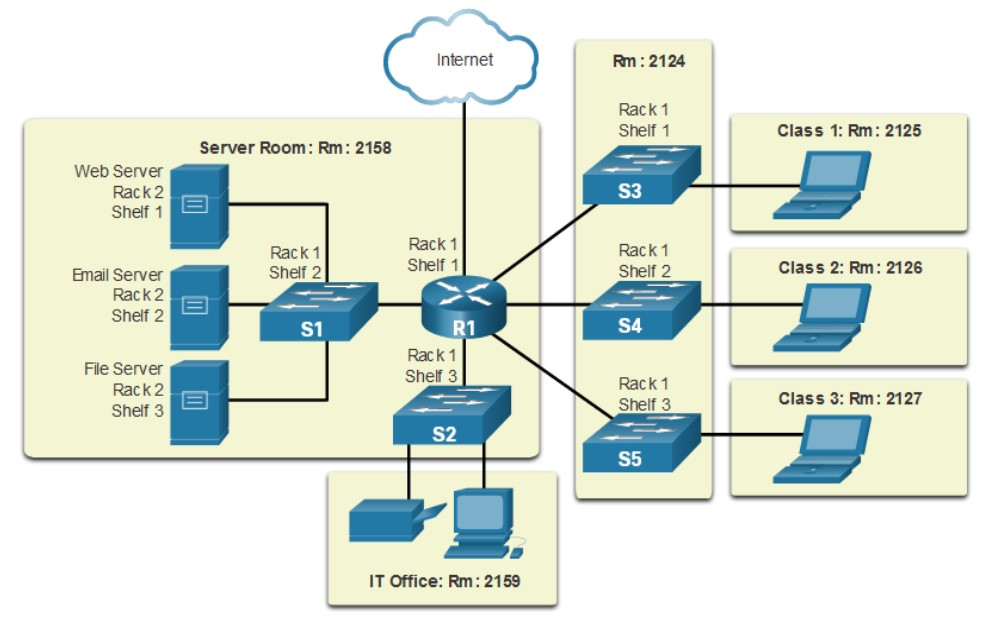
\includegraphics[width=\textwidth]{images/physical_topology_diagram.jpg}
    \caption{Physikalisches Netzwerkdiagramm (\textsuperscript{\textcopyright}Cisco)}
    \end{center}
\end{figure}
\paragraph{Das logische Netzwerkdiagramm}zeigt hingegen über welche \textsl{\textbf{Ports (interfaces)}} die Komponenten angeschlossen sind, sowie welche \textsl{\textbf{Netzwerkadressierung}} gegeben wurde. Merkmale sind Netzwerkadressen, IP-Adressen von Endgeräten, Subnetzmasken, je nach Anwendung auch MAC-Adressen\footnote{Media-Access-Control}. Man spricht auch von einer \textsl{physischen Adresse} oder \textsl{Geräteadresse}.
\begin{figure}[H]
    \begin{center}
    \label{pic:logical_topology}
    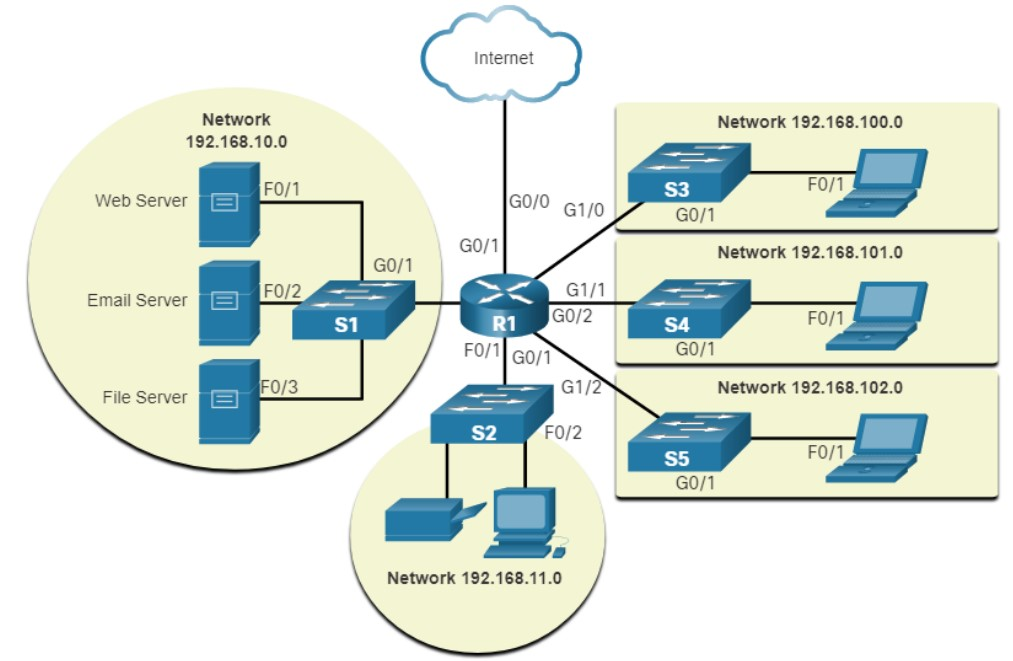
\includegraphics[width=\textwidth]{images/logical_topology_diagram.jpg}
    \caption{Logisches Netzwerkdiagramm (\textsuperscript{\textcopyright}Cisco)}
    \end{center}
\end{figure}
\subsection*{Wie kann man anhand ihrer Grösse Computernetzwerke klassifizieren?}
Es gibt diverse Grössen von Netzwerke. Namentlich sind das:
\begin{itemize}
    \item LAN - Local Area Network. Lokales Netz, mal abgesehen von Subnetzen, auf die Wohnung, Büro oder Firma beschränkt.
    \item MAN - Metropolitan Area Network. Meistens ein Verbund von LANs, welche auf ``kürzere Distanzen'' (bis zu ca. 100 km) durch einen Backbone (Netz mit besonders grosser Übertragungsrate über Glasfaser) vernetzt sind. MANs werden durch Internetdienstanbieter (ISP - Internet Service Provider) betrieben.
    \item WAN - Wide Area Network. Verbund und Backbone von MANs. Salopp: ``Ze Internet''.
\end{itemize}
Die Aufzählung ist nicht abschliessend, denn es gibt z.B. Body Area Network (z.B. medizinische Geräte), Personal Are Network (z.B. Bluetooth), City Area Network, Global Area Network etc.
\subsection*{Wie unterschieden sich LANs und WANs? Was ist ihre Beziehung?}
Sie pflegen eine versteckte Beziehung. Kann ihre Liebe so weiterlodern, inmitten von Intrigen, Verrat und Krieg zwischen den Königshäusern?
\subsection*{Was ist das Internet? Wer besitzt das Internet? Was für Organisationen sind in der Entwicklung des Internets beteiligt?}
Das Internet ist ein globaler Verbund von Rechnernetzwerken, welches die Nutzung von diversen Diensten wie WWW, Email, FTP u.v.m. bietet. Das Internet gehört im Grunde genommen niemandem. Die Organisation IETF\footnote{Internet Engineering Task Force} befasst sich jedoch mit der Weiterentwicklung des Internets, um dessen Funktionsweise zu verbessern.\footnote{\url{https://www.facebook.com/Ballybegpostofficeandgeneralconveniencestore/videos/845703122288697/}}
\subsection*{Was ist der Unterschied zwischen einem Intranet und einem Extranet?}
Auf das Intranet kann nur von innerhalb des LANs zugegriffen werden. Das Extranet bietet hingegen eine Erweiterung des Intranets, die von einer Gruppe von externen Benutzer verwendet werden darf. Extranets bieten Informationen die z.B. an Kunden oder Partnern zugänglich gemacht werden.
\subsection*{Wie verbinden sich normalerweise Häuser, Wohnungen und HomeOffices mit dem Internet?}
Kabelnetz, DSL - Digital Subscriber Line, Dial-Up Modem, GSM - Global System for Mobile Communications, Satellit.
\subsection*{Wie verbinden sich normalerweise Büros und Unternehmern mit dem Internet?}
Dedicated Leased Lines, Metro Ethernet (ethernetbasierte MANs), Business DSL, Satellit.
\subsection*{Was bedeutet Konvergenz im Kontext der Computernetzwerke?}
Voneinander getrennte Netze werden zusammengeführt. Bsp.: klassische Telefonie funktioniert zunehmend über VoIP (Voice over IP).

\begin{figure}[H]
    \begin{center}
    \label{pic:converging_classic}
    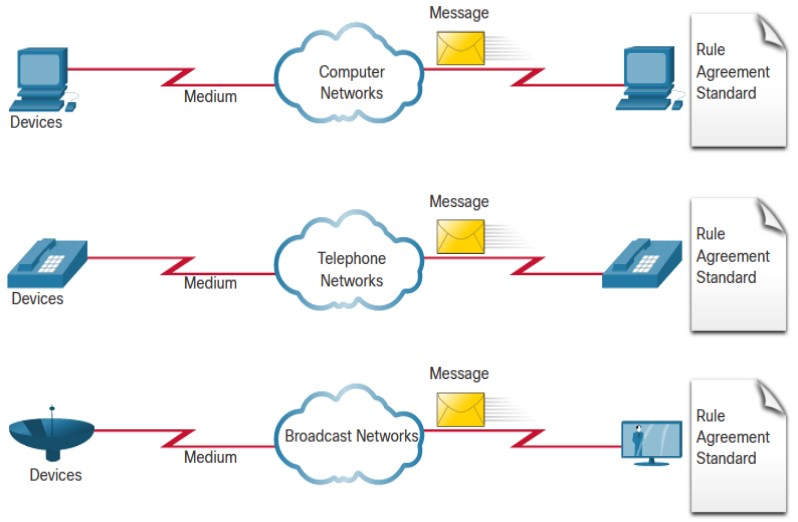
\includegraphics[width=.6\textwidth]{images/converging_network_classic.jpg}
    \caption{Klassisches Netz (\textsuperscript{\textcopyright}Cisco)}
    \end{center}
\end{figure}
\begin{figure}[H]
    \begin{center}
    \label{pic:converging_modern}
    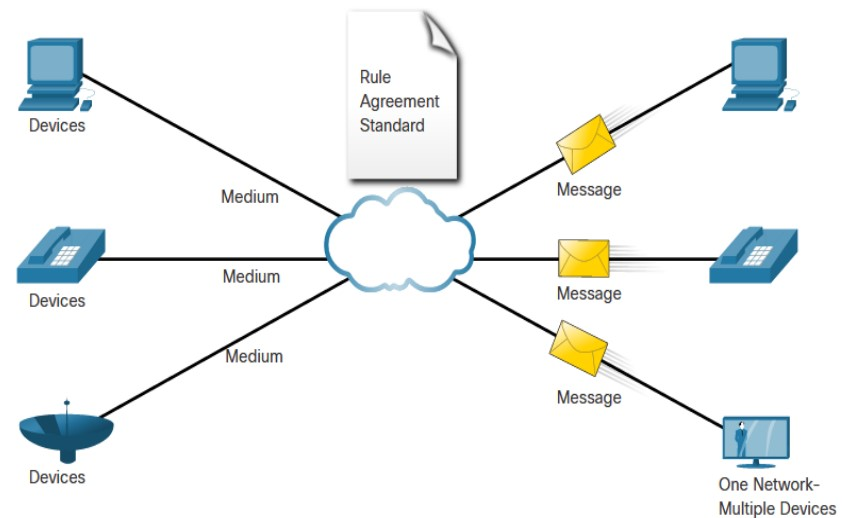
\includegraphics[width=.6\textwidth]{images/converging_network_modern.jpg}
    \caption{Modernes, konvergiertes Netz (\textsuperscript{\textcopyright}Cisco)}
    \end{center}
\end{figure}
\subsection*{Was bedeutet \flqq fault tolerance\frqq{} (Fehlertoleranz) im Kontext der Computernetzwerke? Geben Sie ein Beispiel}
Beim Ausfall einer wichtigen Netzwerkkomponente wie z.B. Router, wird mit redundantem Aufbau eines Netzwerkes die Verbindung weiterhin gewährleistet.
\begin{figure}[H]
    \begin{center}
    \label{pic:fault_tolerance}
    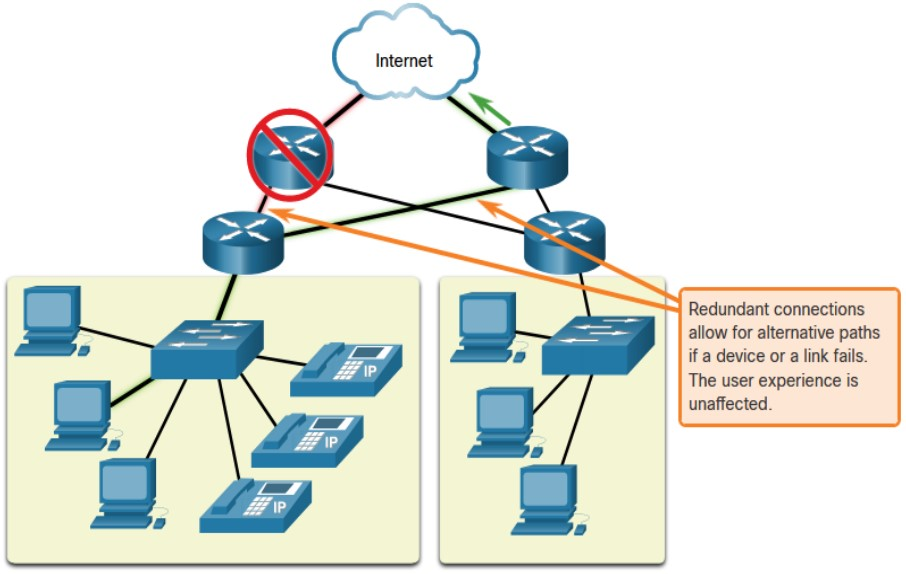
\includegraphics[width=\textwidth]{images/fault_tolerance.jpg}
    \caption{Fault tolerance - Fehlertoleranz (\textsuperscript{\textcopyright}Cisco)}
    \end{center}
\end{figure}
\pagebreak
\subsection*{Was bedeutet \flqq scalability\frqq{} (Skalierbarkeit) im Kontext der Computernetzwerke? Geben Sie ein Beispiel}
Die Skalierbarkeit eines Netzwerkes beschreibt die Fähigkeit/Möglichkeit, ein Netzwerk ohne grossen Aufwand zu erweitern.
\begin{figure}[H]
    \begin{center}
    \label{pic:scalability}
    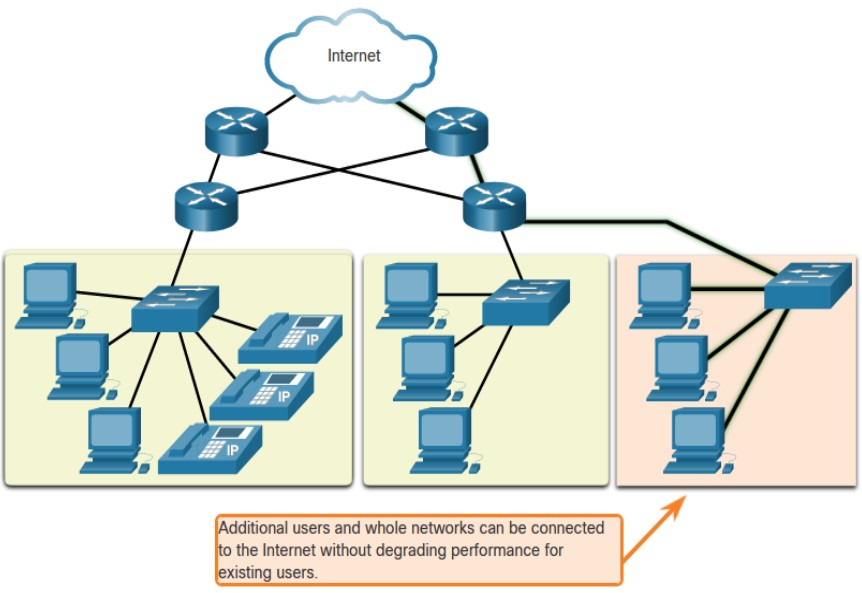
\includegraphics[width=\textwidth]{images/scalability.jpg}
    \caption{scalability - Skalierbarkeit (\textsuperscript{\textcopyright}Cisco)}
    \end{center}
\end{figure}
\subsection*{Was bedeutet \flqq quality of service (QoS)\frqq{} im Kontext der Computernetzwerke? Geben Sie ein Beispiel}
Das QoS dient zur Priorisierung von Netzwerkdiensten und -paketen. Ein Telefonat über VoIP ist wichtiger als eine Webseite, die vielleicht ein paar Millisekunden länger braucht um angezeigt zu werden.
\begin{figure}[H]
    \begin{center}
    \label{pic:qos}
    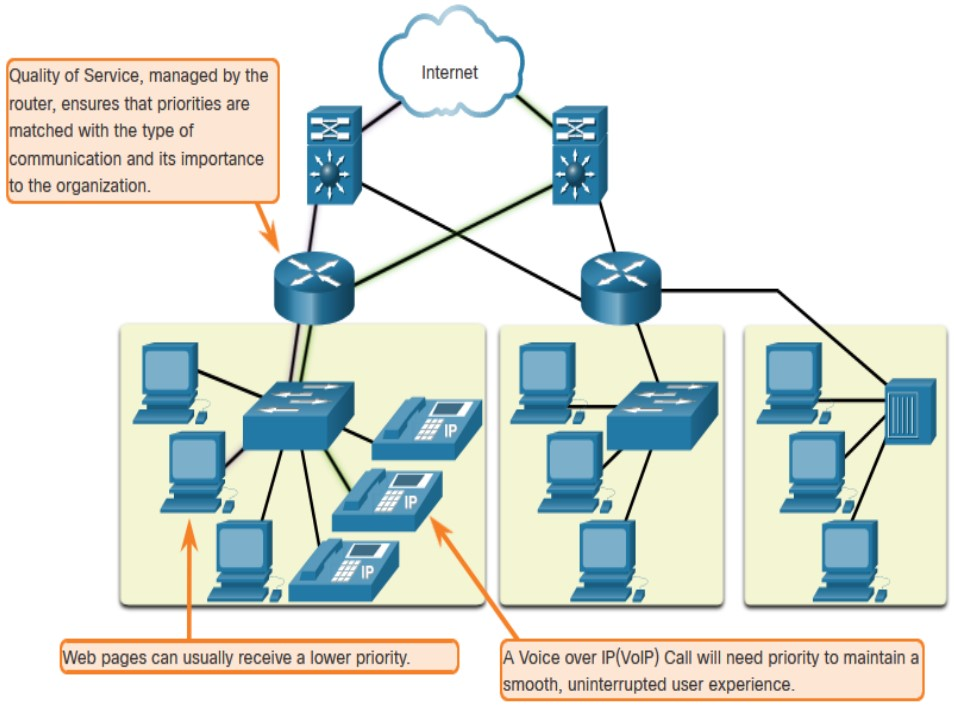
\includegraphics[width=\textwidth]{images/qos.jpg}
    \caption{Quality of service}
    \end{center}
\end{figure}
\subsection*{Wieso ist Netzwerksicherheit wichtig?}
Um Unbefugten nicht versehentlichen oder absichtlichen Zugriff auf das Netzwerk zu gewähren.
\subsection*{Was sind die drei Hauptinformationssicherheitsziele?}
Informationssicherheit ist das höchste Gut, der heilige Grahl der Informatik. Die drei Hauptziele sind:
\begin{itemize}
    \item \textbf{Vertraulichkeit} (confidentiality): lediglich autorisierte Benutzer dürfen entsprechende Daten lesen (z.B. eavesdropper) oder ändern. Dies gilt beim Zugriff auf gespeicherte Daten, wie auch während der Übertragung.
    \item \textbf{Integrität} (integrity): Daten dürfen nicht unbemerkt verändert werden (z.B. man in the middle attack) und alle Änderungen müssen nachvollziehbar sein.
    \item \textbf{Verfügbarkeit} (availability): Verhinderung von Systemausfällen und Gewährleistung der Verfügbarkeit der Daten innerhalb eines definierten Zeitraums.
\end{itemize}
Informationssicherheit wird im Modul ISF - Information Security Fundamentals genauer erarbeitet.
\subsection*{Was ist \flqq BYOD\frqq{} und was sind seine Auswirkungen für Geschäfte und Unternehmen?}
Bring Your Own Device. Für Unternehmen bedeutet dies, dass Komponenten wie Smartphones und Notebooks in das Netzwerk eingebunden werden, welche vielleicht nicht über spezielle Schutzmassnahmen verfügen, als wenn es von der firmeneigenen Informatikabteilung zur Verfügung gestellt werden würde. Umso besser muss das Netzwerk gegen mögliche Bedrohungen, die dieses Philosophie mit sich bringt, geschützt werden.
\subsection*{Was ist \flqq cloud computing\frqq{}? Was für Cloud Arten gibt es?}
Clouds sind verschiedene Dienstleistungen, welche physisch nicht mehr verfügbar sind. Bekanntestes Anwendungsbeispiel ist die File-Cloud. Man hat nicht einen eigenen File-Server, sondern einen externen Anbieter, einen CSP - Could Service Provider, der den Zugang auf die darunterliegende Infrastruktur ermöglicht. Im Grunde gibt es drei Hauptformen von Angeboten:
\begin{itemize}
    \item Software as a Service (SaaS)
    \item Platform as a Service (PaaS)
    \item Infrastructure as a Service (Iaas)
\end{itemize}
Wichtig dabei ist, dass es vier verschiedene Arten von Clouds gibt.
\begin{itemize}
    \item Private
    \begin{itemize}
        \item Ein Unternehmen hat Zugriff auf eine Cloud-Infrastruktur, welche nicht von anderen Firmen genutzt wird (z.B. Dedicated Server). Sicher was Datenschutz angeht, jedoch Verfügbarkeit könnte bei einem Ausfall vielleicht nicht gewährleistet sein.
    \end{itemize}
    \item Public
    \begin{itemize}
        \item Ein Unternehmen teilt sich eine Cloud-Infrastruktur mit anderen Firmen (z.B. Shared Server). Das heisst also, eine Firma bekommt eine definierte Anzahl an Ressourcen zur Verfügung gestellt, hat aber keinen Zugriff auf die gesamte Infrastruktur. Normalerweise sehr hohe Verfügbarkeit, jedoch vom Datenschutz her nicht optimal, da sich Infrastruktur global befindet (Big Brother is watching you), jedoch deswegen auch günstiger im Angebot.
    \end{itemize}
    \item Hybrid
    \begin{itemize}
        \item Hybride Cloud-Infrastrukturen sind in private und public Clouds geteilt. Sensitive Daten werden in der privaten cloud verarbeitet. Operationen die von sensitiven Daten keinen Gebrauch machen können günstig in einer public Cloud verarbeitet werden. Je nach bedarf kann die public Cloud skaliert werden.
    \end{itemize}
    \item Community
    \begin{itemize}
        \item Die Community Cloud ist eine spezielle Form der Cloud. Spezifische Sektoren wie Gesundheits-, Recht-, Finanzbereich u.a. unterliegen oft regulatorischen Konformitäten. Diese ``Sektorsphären'' sind als die Communities anzusehen. CSPs haben aufgrund dieser Konformitäten ein gewisses Angebotsstandard für die Sektoren geschaffen. Vom Datenschutz fast wie eine private Cloud, jedoch von der Funktionalität wie eine public cloud, das heisst, andere Firmen aus derselben Branche nutzen die Cloud mit.
    \end{itemize}
\end{itemize}

Wie bei allem gibt es Vor- und Nachteile bei der Nutzung solcher Angebote.
\subsection*{Was ist die Verbindung zwischen \flqq cloud computing\frqq{} und Computernetzwerken?}
Cloud Computing ist ein Dienstleitungsangebot von Cloud Service Providern. Ein Computernetzwerk ist die darunterliegende Struktur zur Gewährleistung der Datenübertragung.
\part{SW 02 - ISO/OSI Modell}
\section{Lernziele (Leitfragen)}
\begin{enumerate}
    \item Was sind die Schichten des TCP/IP Models? Beschreiben Sie den Zweck jeder Schicht
    \item Was sind die Schichten des OSI Models? Beschreiben Sie den Zweck jeder Schicht
    \item Was ist die Verbindung zwischen dem TCP/IP Modell und dem OSI Modell?
    \item Nehmen Sie eine typische Netzwerkapplikation als Beispiel. Anhand des TCP/IP Models, erläutern Sie wie Nachrichten zwischen den End-Devices ausgetauscht sind.
    \item Wieso muss man Zahlensysteme verstehen, wenn man sich mit Computernetzwerken beschäftigt?
    \item Wie kann man einfach und schnell zwischen Binär, Hexadezimal und Dezimal umrechnen?
\end{enumerate}

\section{Antworten}
\subsection*{Was sind die Schichten des TCP/IP Models? Beschreiben Sie den Zweck jeder Schicht}\index{Modell!TCP/IP}
Das TCP/IP Modell besteht aus vier Schichten.\\
Eselsbrücke: \underline{$\mathbb{A}$}lle \underline{$\mathbb{T}$}iere \underline{$\mathbb{I}$}n \underline{$\mathbb{N}$}oah's \underline{$\mathbb{A}$}rche\\

\begin{table}[H]
\begin{tabularx}{\textwidth}{|c|X|l|}
    \multicolumn{1}{c}{Layer}&\multicolumn{1}{X}{Zusammenfassung}&\multicolumn{1}{l}{Protokolle}\\
    \hline
    \makecell[c]{Application}&\makecell[X]{- Am nächsten zum User\\- Datenaustausch zwischen Programmen\\- Allgemeine Funktionen zur Kommunikation im Internet}&\makecell[l]{Web (HTTP, HTTPS)\\Email (POP, IMAP, SMTP)\\Namensauflösung (DNS)\\Datenaustausch (FTP)}\\
    \hline
    \makecell{Transport}&\makecell[X]{- Segmentierung und Zusammenfügen von Daten\\- Management von Verlässlichkeitsanforderungen einer Konversation\\- Multiplexing und Konversationen verfolgen}&\makecell[l]{Verbindungsorierntiert (TCP)\\Verbindungslos (UDP)}\\
    \hline
    \makecell{Internet}&\makecell[X]{- Datenaustausch über Sub-Netzwerke\\- Adressierung von Endgeräten\\- Routing\\- verbindungslos, best effort und medienunabhängig}&\makecell[l]{Datenaustausch (IPv4, IPv6)\\Routing (OSPF, BGP)\\Steuerung (ICMPv4, ICMPv6)}\\
    \hline
    \makecell{Network\\Access}&\makecell[X]{- Adressierung von Sub-Netzwerken\\- Media access control (MAC)\\- Abstraktion der physischen Medien der oberen Schichten\\- Bits auf die Medien setzen}&\makecell[l]{Address Resolution (ARP)\\Data Link (Ethernet, WLAN)}\\
    \hline
\end{tabularx}
\caption{TCP/IP Modell}
\end{table}

\subsection*{Was sind die Schichten des OSI Models? Beschreiben Sie den Zweck jeder Schicht}\index{Modell!OSI}\label{sub:SchichtenOSIModell}
Das OSI Modell besteht aus 7 Schichten.\\
Eselsbrücke: \underline{$\mathbb{A}$}lle \underline{$\mathbb{P}$}riester \underline{$\mathbb{S}$}aufen \underline{$\mathbb{T}$}equilla \underline{$\mathbb{N}$}ach \underline{$\mathbb{D}$}er \underline{$\mathbb{P}$}redigt\\

\begin{table}[H]
\begin{tabularx}{\textwidth}{|c|X|c|}
    \multicolumn{1}{c}{Layer}&\multicolumn{1}{X}{Zusammenfassung}&\multicolumn{1}{l}{Protokolle}\\
    \hline
    \multicolumn{3}{|c|}{$\downarrow$Anwendungsorientiert$\downarrow$}\\
    \hline
    \makecell[c]{Layer VII\\Anwendungen\\(Application)}&\makecell[X]{Die Anwendungsschicht interagiert direkt mit der Software (Anwendung), die eine Netzwerkübertragung anfordert. Sie ermittelt, ob die Möglichkeit einer Verbindung besteht, und identifiziert und sucht Ressourcen.}&\multirow{12}{*}{\makecell[c]{DHCP\\DNS\\FTP\\HTTPS\\LDAP\\SMTP\\\dots}}\\
    \cline{1-2}

    \makecell[c]{Layer VI\\Darstellung\\(Presentation)}&\makecell[X]{Die Darstellungsschicht sorgt dafür, dass die Daten so bearbeitet werden, dass sie optimal ausgetauscht und verarbeitet werden können. Hierfür gibt es etliche standardisierte Kodierungs-, Konvertierungs- und Kompressionsverfahren, zum Beispiel für Verschlüsselungsroutinen, Zeichendarstellungen, Video- und Audioübertragungen.}&\\
    \cline{1-2}

    \makecell[c]{Layer V\\Kommunikations-/\\Sitzungsschicht\\(Session)}&\makecell[X]{Die Kommunikationsschicht ist hauptsächlich eine "`Serviceschicht"' für die bidirektionale Kommunikation von Anwendungen in verschiedenen Endgeräten. Sitzungen und Datenströme werden angefordert, aufgebaut, kontrolliert und koordiniert. Meist bedienen sich die Services der Schicht 5 dabei der Dienstangebote der Schicht 4.}&\\
    \hline

    \makecell[c]{Layer IV\\Transportschicht\\(Transport)}&\makecell[X]{In der Transportschicht sind Sicherungsmechanismen für einen zuverlässigen Datentransport beschrieben. Die Schicht 4 regelt das Datenmultiplexing und die Flusskontrolle, das heisst, mehrere Anwendungen höherer Protokolle können gleichzeitig Daten über eine Verbingdung tranportieren. In der Tranportschicht sind verbindugslose und verbindungsorientierte Dienste implementiret. Verbindungsorientierte Diense können einen sehr sicheren Datenaustausch durchführen. Der Sender und der Empfänger kontrollieren ihre Möglickeiten der Kommunikation (Aufbau einer virtuellen Verbindung), die Daten werden erst nach dieser Prfung versandt. Eine weitgehende Fehlerkontrolle prüft die Daten und fordert entweder verlorene oder korrumpierte Daten zur erneuten Übersendung an. Am Ende der Kommunikation wird die Verbindung gezielt und kontrolliert wieder abgebaut. Im Layer 4 wird nach definierten Anwendungen unterschieden. Hier beginnt die Kommunikation zwischen dem Netzwerk un der Anwendung.}&\makecell[c]{TCP\\UDP\\\dots}\\
    \hline

    \multicolumn{3}{|c|}{$\downarrow$Transportorientiert$\downarrow$}\\
    \hline

    \makecell[c]{Layer III\\Vermittlungsschicht\\(Network)}&\makecell[X]{In der Schicht 3 des OSI-Modells wird die logische Adressierung (segmentübergreifend bis weltweit) der Geräte definiert. Die Routing-Protokolle dieser Schicht ermöglichen die Wegfindung in grossen (bis weltweiten) Netzwerken und redundante Wege ohne Konflikte. Routing-Protokolle sorgen ebenfalls dafür, dass die Ressourcen in vermaschten Netzen mit vielen redundanten Wegen bei dem Ausfall einer Verbindung weiterhin benutzt werden können.}&\makecell[c]{ICMP\\IP\\IPsec\\IPX\\\dots}\\
    \hline

    \makecell[c]{Layer II\\Sicherungsschicht\\(Data Link)}&\makecell[X]{Die Sicherungsschicht ist für eine zuverlässige Übertragung der Daten zuständig. Sie regelt die Flusssteuerung, regelt den Zugriff, verhindert eine Überlastung des Empfängers und ist für die physikalische Adressierung innerhalb eines Netzsegmentes auf dieser Schicht verantwortlich. Hier ist die erste Fehlererkennung implementiert. Die Topologie eines Netzwerkes ist stark von dieser Schicht abhängig, sie definiert die Art und Weise, wie die Rechner und Netzwerkgeräte miteinander verbunden sind.}&\makecell[c]{IEEE 802.3\\(Ethernet)\\IEEE 802.11\\(WLAN)\\MAC\\\dots}\\
    \hline

    \makecell[c]{Layer I\\Physikalische Schicht\\(Physical)}&\makecell[X]{Hier sind die physikalischen Parameter definiert. Dazu gehören Kapeltypen, die Anschlüsse, die Streckenlängen, die elektrischen Eckdaten wie Spannungen, Frequenzen etc. Getrennt wird hier in drei Bereiche:\\\begin{itemize}
        \item Der Nahbereich (LAN)
        \item mittlere Entfernungen (MAN)
        \item und Fernverbindungen (WAN).
    \end{itemize}}&\makecell[c]{1000BASE-T\\10BASE-T\\Token Ring\\\dots}\\
    \hline

\end{tabularx}
\caption{OSI Modell\cite{Schreiner2019}}
\end{table}
\subsection*{Was ist die Verbindung zwischen dem TCP/IP Modell und dem OSI Modell?}\label{sub:VerbindungTCPundOSIModell}
\begin{figure}[H]
    \begin{center}
    \label{pic:osi_tcpip}
    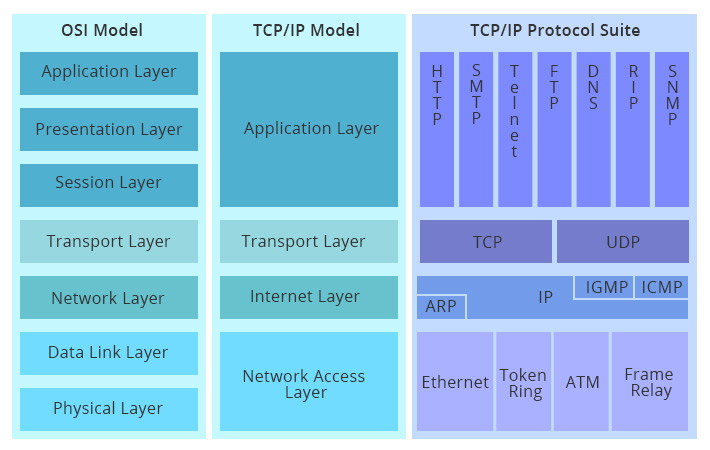
\includegraphics[width=\textwidth]{images/osi_tcpip.jpg}
    \caption[Vergleich OSI mit TCP/IP Modell]{Vergleich OSI mit TCP/IP Modell\cite{FSDeutschland}}
    \end{center}
\end{figure}

\subsection*{Nehmen Sie eine typische Netzwerkapplikation als Beispiel. Anhand des TCP/IP Models, erläutern Sie wie Nachrichten zwischen den End-Devices ausgetauscht sind.}\label{sub:BeispielNetzwerkapplikation}
\begin{figure}[H]
    \begin{center}
    \label{pic:tcp1}
    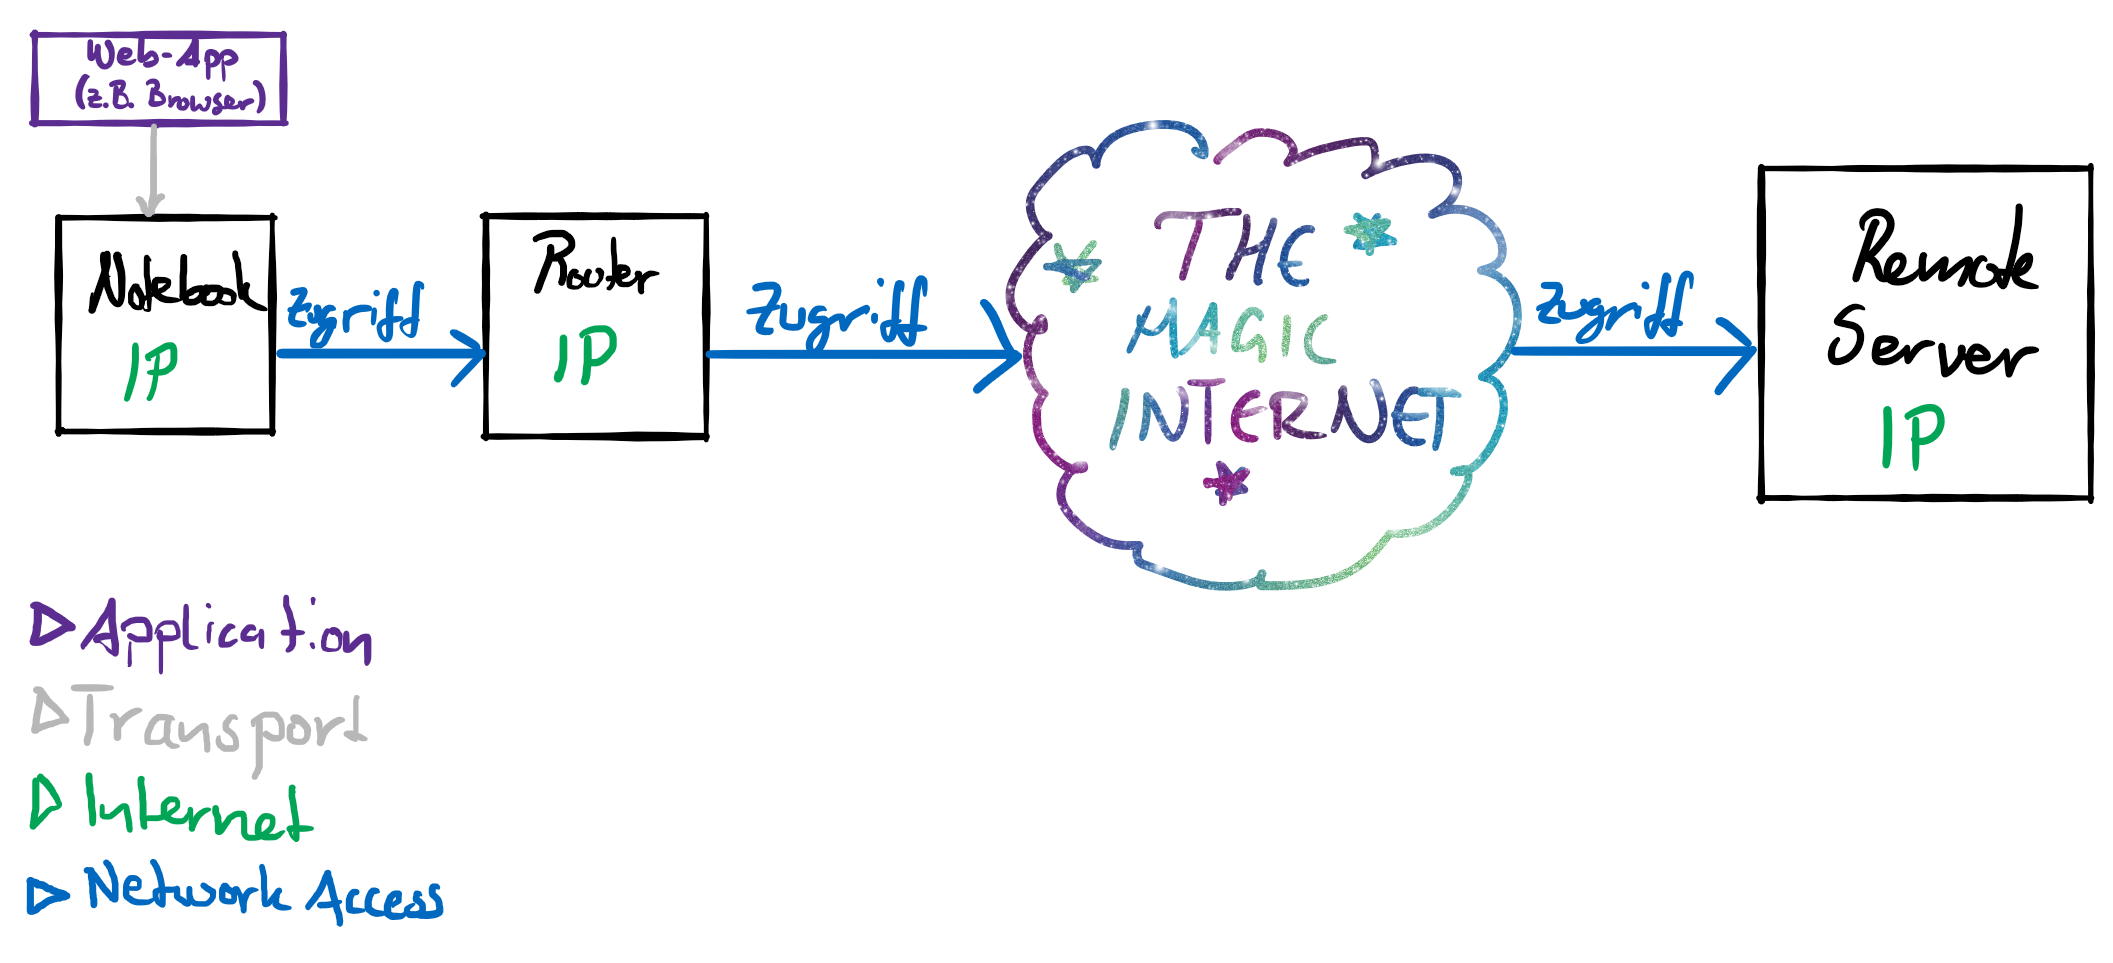
\includegraphics[width=\textwidth]{images/Nachrichtenaustausch01.png}
    \caption{Weg eines Datenpaketes}
    \end{center}
\end{figure}

\begin{figure}[H]
    \begin{center}
    \label{pic:tcp2}
    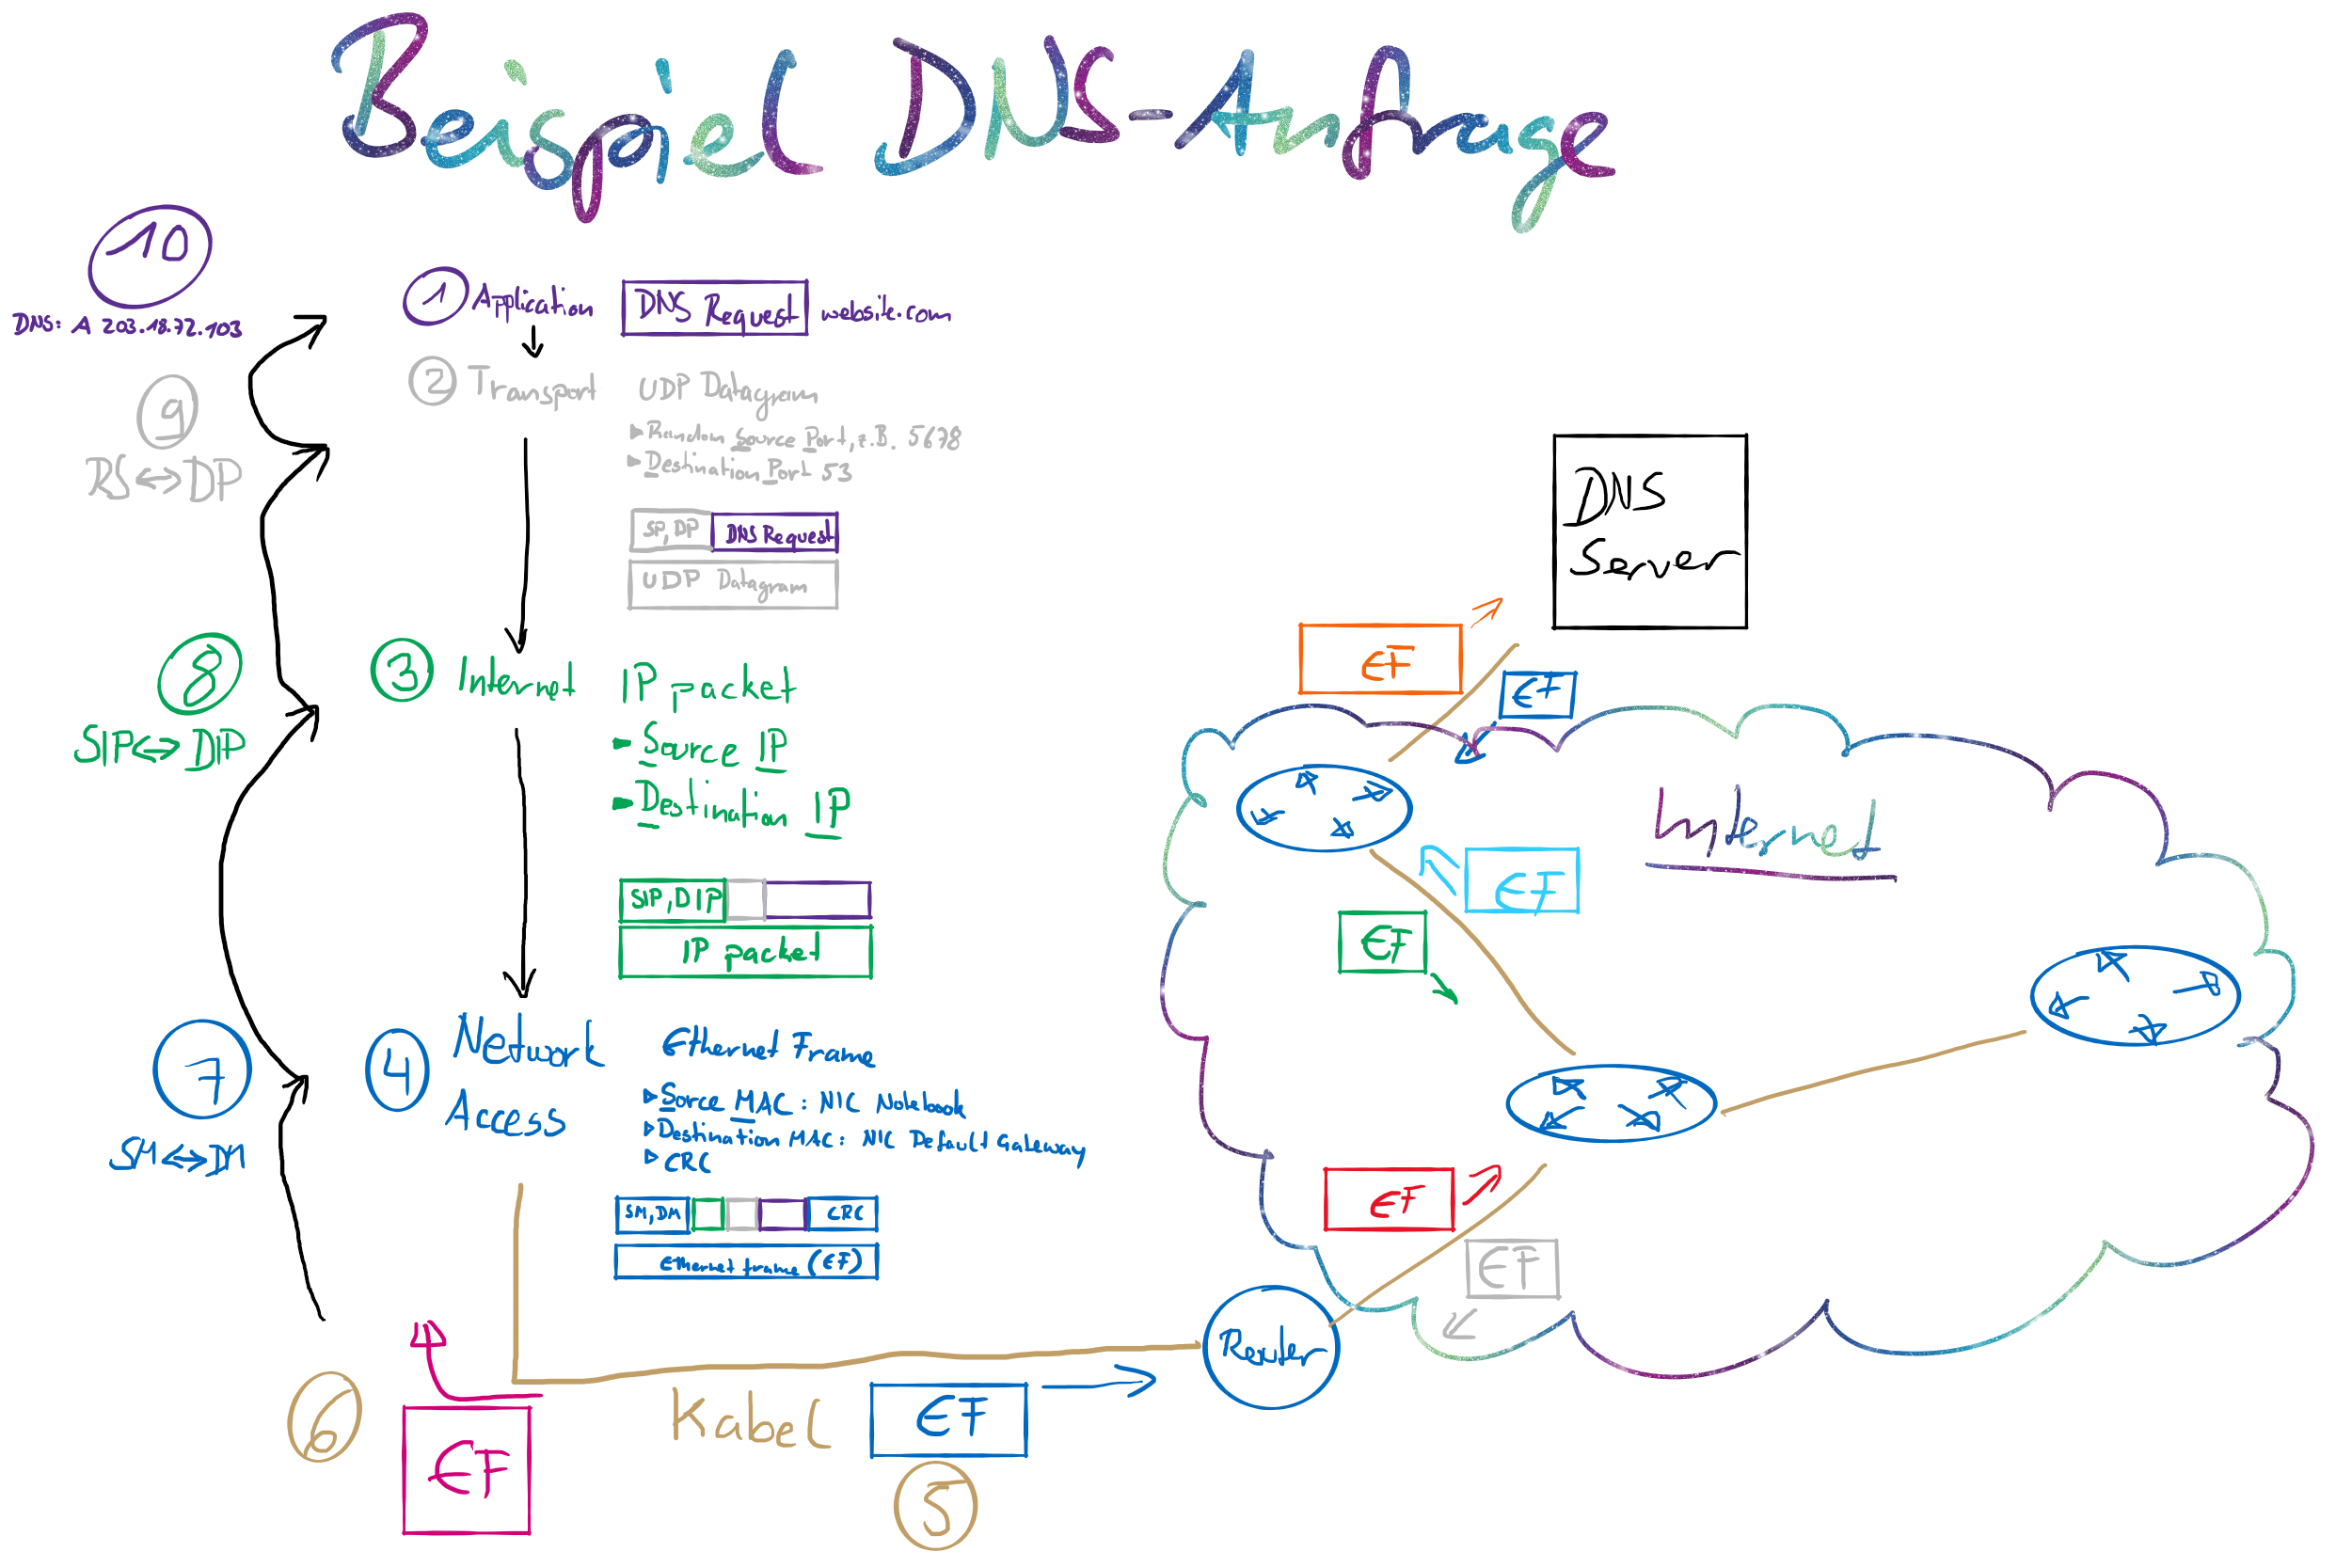
\includegraphics[width=\textwidth]{images/Nachrichtenaustausch02.png}
    \caption{Einzelschritte der Kapselung, Beispiel anhand DNS request}
    \end{center}
\end{figure}

\subsection*{Wieso muss man Zahlensysteme verstehen, wenn man sich mit Computernetzwerken beschäftigt?}\label{sub:ZahlensystemeVerstehen}
Das Rechnen mit anderen Zahlensystemen wie Binär ist im Umgang mit Computernetzwerken insofern wichtig, weil gewisse Rechnungen (z.B. Subnetz) einfacher sind. Auch sind gewisse Zahlen in anderen Formaten dargestellt wie MAC-Adressen oder IPv6, welche in Hexadezimal dargestellt werden, weil diese kompakter sind als Dezimal.

\pagebreak
\subsection*{Wie kann man einfach und schnell zwischen Binär, Hexadezimal und Dezimal umrechnen?}\label{sub:RechnenBinHexDez}
    Über den Rechner vom Betriebssystem:
    \begin{figure}[H]
        \begin{center}
        \label{pic:calc}
        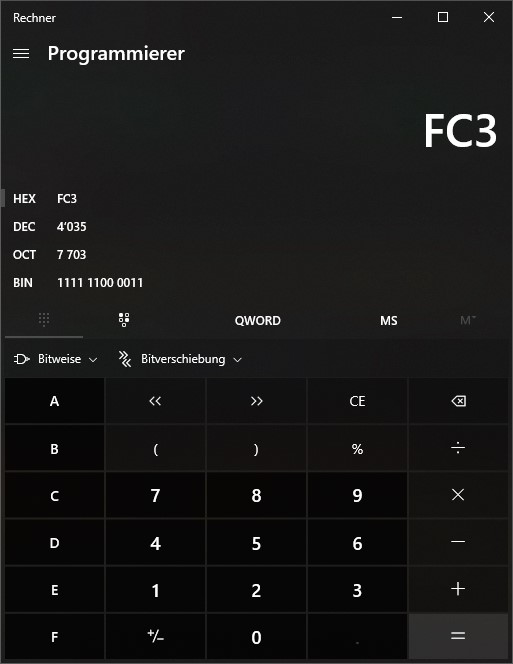
\includegraphics[width=.5\textwidth]{images/calc.jpg}
        \caption{Windows Taschenrechner}
        \end{center}
    \end{figure}
    Oder ganz easy von Hand ausrechnen.
    \paragraph{Binär}Beispiel $125_{10}$ zu Binär. Den Rest zusammenfügen:\\
    \begin{tabular}{rcll}
        125&$\div$&2 = 62&R 1 (ganz rechts)\\
        62&$\div$&2 = 31&R 0\\
        31&$\div$&2 = 15&R 1\\
        15&$\div$&2 = 7&R 1\\
        7&$\div$&2 = 3&R 1\\
        3&$\div$&2 = 1&R 1\\
        1&$\div$&2 = 0&R 1 (ganz links)\\[1em]
\end{tabular}
Dann ist das Ergebnis also: 0b111 1101\\[1em]
Um die Binärzahl in Dezimal umzuwandeln, liest man von rechts die Einsen und fängt mit der Potenz 0 zur Basis 2 an. Unser Zahlenbeispiel als Byte:\\[1em]
\begin{tabular}{cccccccc}
    $2^7$&$2^6$&$2^5$&$2^4$&$2^3$&$2^2$&$2^1$&$2^0$\\
    0&1&1&1&1&1&0&1\\
\end{tabular}\\[1em]
Daraus erhält man, dort wo eine 1 steht:\\$2^6+2^5+2^4+2^3+2^2+2^0=64+32+16+8+4+1=125$.

\pagebreak
\paragraph{Hexadezimal}Hexadezimal ist da schon etwas komplizierter, aber machbar. Hier rechnet man auch mit Potenzen zur Basis 16. Dazu muss man vorgängig aber schon das $16^x$ unterhalb der Zahl kennen.\\
$16^2=256$ ist also zu hoch für unsere 125. Bleibt also die nächst tiefere Potenz  $16^1=16$.\\
Wir teilen also mit 16:\\
\begin{tabular}{rcllll}
    125&$\div$&16&($16^1$)&= 7 (ganz links)&R  13 (mit nächst tiefere Potenz teilen)\\
    13&$\div$&1&($16^0$) &= 13&\\[1em]
\end{tabular}\\
Also hat man jetzt $7\times16^1+13\times16^0$. Das Hexadezimalsystem geht ja aber von 0-F, somit ist die 13 ein D (\dots, 9, 10=A, 11=B, 12=C, 13=D, 14=E, 15=F). Das Ergebnis ist als 0x7D. Auch easy.\\[1em]
Umgekehrt von Hexadezimal auf Dezimal umzurechnen, folgt man dem nun bekannten Potenz-Prinzip.\\$7\times16^1+13\times16^0=125_{10}$\\[1em]
Hexadezimal und Binär ist Bubieinfach. Dazu nimmt man Binär halbe Bytes (Nibble) und stellt die Zahlen gegenüber.\\
\begin{tabular}{cccc|cccc}
    $2^3$&$2^2$&$2^1$&$2^0$&$2^3$&$2^2$&$2^1$&$2^0$\\
    0&1&1&1&1&1&0&1\\
    \hline
    \multicolumn{4}{c|}{7}&\multicolumn{4}{c}{13 = D}\\
\end{tabular}\\[1em]

Was ist mit grossen Zahlen? Dazu brauchen wir einen Taschenrechner mit der Log-Funktion. Nehmen wir als Beispiel $1'106'132_{10}$. Um die Potenz $x$ von $16^x$ herauszufinden, logarithmieren wir diese Zahl mit dem Taschenrechner: $\frac{\log{1106132}}{\log{16}}=5.00000103189442\dots$ \\
Wir wissen nun, das es sich beim Exponenten um die Potenz 5 handelt. Teilen die Zahl mit $16^5$ und erhalten $1.0548\dots$ Wir subtrahieren die 1 vom Ergebnis und die Nachkommastellen$\times$\underline{Divisor} (hier $16^5$) ergeben den Rest von 57556. Den Rest wieder logarithmieren für nächste Potenz u.s.w. Wir rechnen nun (Zwischenschritt für Rest und Potenz nicht dabei):\\
\begin{tabular}{rcllll}
    1106132&$\div$&1048576&($16^5$)&= 1 (ganz links)&R 57556 (mit nächst tiefere Potenz teilen)\\
    57556&$\div$&4096&($16^3$)&= 14&R 212\\
    212&$\div$&16&($16^1$)&= 13&R 4\\
    4&$\div$&1&$(16^0)$&= 4&R 0\\[1em]
\end{tabular}\\

Nun können wir überall dort, wo ein Exponent steht, die Zahl Schreiben. Überall dort wo kein Exponent ist (hier: 4, 2), wird 0 geschrieben:\\
\begin{tabular}{cccc|c|cccc|c|cccc|cccc}
    $2^3$&$2^2$&$2^1$&$2^0$&&$2^3$&$2^2$&$2^1$&$2^0$&&$2^3$&$2^2$&$2^1$&$2^0$&$2^3$&$2^2$&$2^1$&$2^0$\\
    0&0&0&1&0000&1&1&1&0&0000&1&1&0&1&0&1&0&0\\
    \hline
    \multicolumn{4}{c|}{1}&\multicolumn{1}{c|}{0}&\multicolumn{4}{c|}{14 = E}&\multicolumn{1}{c|}{0}&\multicolumn{4}{c|}{13 = D}&\multicolumn{4}{c}{4}\\
\end{tabular}\\[1em]
Das Ergebnis ist also 0x10E0D4, Binär 0b0001 0000 1110 0000 1101 0100.\\[1em]
Hexadezimal zu Dezimal wie vorhin bereits beschrieben: $1\times16^5+14\times16^3+13\times16^1+4\times16^0=1106132_{10}$
\part{SW 03 - Präsentationen zu physikalischer Schicht}
\section{Lernziele (Leitfragen)}
\begin{itemize}
    \item Die physikalische Schicht und Zugriffsverfahren (T1)
    \begin{enumerate}
        \item Was ist der Zweck der physikalischen Schicht?
        \item Was sind die Hauptmerkmale der physikalischen Schicht?
        \item Was ist der Unterschied zwischen \flqq{}Simplex\frqq, \flqq{}half-duplex\frqq{} and \flqq{}full duplex\frqq?
        \item Welches sind die am häufigsten verwendeten Zugriffsverfahren?
        \item Was ist der Unterschied zwischen CSMA/CD und CSMA/CA? Wo werden sie verwendet?
        \item Was bedeutet "`Late Collision"'?
        \item Was muss man noch unbedingt über die physikalische Schicht und Zugriffsverfahren wissen?\\
    \end{enumerate}

    \item Topologien und "`Bandwidth"' (T2)
    \begin{enumerate}
        \item Was für Topologien findet man in Computernetzwerken?
        \item Wo ist der Unterschied zwischen \flqq{}Bandwidth\frqq, \flqq{}Throughput\frqq{} und \flqq{}Goodput\frqq? Wie kann man diese Konzepte visualisieren und verstehen?
        \item Was ist \flqq{}Latency\frqq{} und \flqq{}Jitter\frqq? Wie kann man diese Konzepte visualisieren und verstehen?
        \item Was muss man noch unbedingt über Topologien und "`Bandwidth"' wissen?\\
    \end{enumerate}

    \item Kupferkabel (T3)
    \begin{enumerate}
        \item Was sind die wichtigsten Merkmale von Kupferkabeln?
        \item Was für Kupferkabelarten werden heutzutage in Computernetzwerken am häufigsten verwendet?
        \begin{enumerate}
            \item Wie sind sie aufgebaut?
            \item Wie sehen die Stecker aus?
        \end{enumerate}
        \item Worauf muss bei der Handhabung und Verlegung der Kupferkabel besonders geachtet werden und warum?
        \item Woraus resultieren die Längenbeschränkungen der Kupferverkabelung?
        \item Was muss man noch unbedingt über Kupferkabel wissen?\\
    \end{enumerate}

    \item Glasfaserkabel (T4)
    \begin{enumerate}
        \item Was sind die wichtigsten Merkmale von Glasfaserkabeln?
        \begin{enumerate}
            \item Wie sind sie aufgebaut?
            \item Wie sehen die Stecker aus?
        \end{enumerate}
        \item Worauf muss bei der Handhabung und Verlegung von Glasfaserkabeln besonders geachtet werden und warum?
        \item Woraus resultieren die Längenbeschränkungen der Glasfaserkabelverkabelung?
        \item Wo ist der Unterschied zwischen Multi- und Singlemode (Monomode)- Glasfasern?
        \item Was sind die Vor- und Nachteile von Glasfaserkabel (im Vergleich zu Kupferkabeln)?
        \item Was muss man noch unbedingt über Glasfaserkabel wissen?\\
    \end{enumerate}

    \item Wireless Access (T5)
    \begin{enumerate}
        \item Was sind die wichtigsten Merkmale von \flqq{}Wireless Media\frqq?
        \item Welche Wireless Access Geräte arbeiten auf Layer I?
        \item Was für Wireless Standards gibt’s in Computernetzwerken?
        \begin{enumerate}
            \item Was sind ihre Hauptmerkmale und Anwendungsbereiche?
        \end{enumerate}
        \item Was sind die Vor- und Nachteile von \flqq{}Wireless Access\frqq{} Methoden im Vergleich mit \flqq{}Wired Access\frqq?
    \end{enumerate}
\end{itemize}

\section{Antworten T1}
\subsection*{Was ist der Zweck der physikalischen Schicht?}
\begin{itemize}
    \item Bietet elektrische, mechanische und funktionale Schnittstelle zum Medium
    \item Definiert die Grösse der Bits (Geschwindigkeit)
    \item Definiert die Art der Übertragung und Codierung (z.B. elektromagnetische Wellen)
    \item Kommunikation zwischen Übertragungsmedien
    \begin{itemize}
        \item Lichtwellenleiter
        \item Stromkabel
        \item Stromnetz
    \end{itemize}
\end{itemize}

\subsection*{Was sind die Hauptmerkmale der physikalischen Schicht?}\index{Schichten!Physikalicshe Schicht}
\begin{itemize}
    \item Digitale Bit-Übertragung: \textsl{funktioniert indem...}
    \begin{itemize}
        \item \textsl{\dots{}über Kabel\dots}
        \begin{itemize}
            \item Kupfer, Lichtwellenleiter, Stromnetz
        \end{itemize}
        \item \textsl{\dots{}eine Verbindung\dots}
        \begin{itemize}
            \item statisches Multiplexing (synchron)
            \item dynamisches Multiplexing (asynchron)
        \end{itemize}
        \item \textsl{\dots{}an die richtigen Steckplätze hergestellt wird.\dots}
    \end{itemize}
    \item Definition der Übertragung eines Bits
    \begin{itemize}
        \item Dabei nicht nur 0 oder 1, sondern mehr
        \begin{itemize}
            \item Lichtintensität (Glasfaser)
            \item Spannung \& Ströme (elektrische Leitung)
            \item Binär (Datenstrom)
        \end{itemize}
        \item Übertragungsart muss mit Codierung versehen werden
    \end{itemize}
\end{itemize}

\subsection*{Was ist der Unterschied zwischen \flqq{}Simplex\frqq, \flqq{}half-duplex\frqq{} and \flqq{}full duplex\frqq?}\index{Kommunikation!Simplex}\index{Kommunikation!Half-Duplex}\index{Kommunikation!Full-Duplex}\index{Simplex}\index{Half-Duplex}\index{Full-Duplex}
Vergleiche Kommunikationsrichtung, das Senden/Empfangen, Leistung und Beispiele:
\begin{itemize}
    \item Simplex
    \begin{itemize}
        \item Unidirektional
        \item Nur Sender schickt Daten
        \item Schlechteste Leistung in Übertragung
        \item Tastatur$\rightarrow$Monitor
    \end{itemize}
    \item Half-Duplex
    \begin{itemize}
        \item Bidirektional: eins auf einmal
        \item Sender kann Daten senden und empfangen, aber nur ein Sender auf einmal
        \item Besser als Simplex
        \item Walkie-Talkie
    \end{itemize}
    \item Full-Duplex
    \begin{itemize}
        \item Bidirektional: alle gleichzeitig
        \item Sender schickt und empfängt Daten gleichzeitig
        \item Beste Leistung
        \item Telefon
    \end{itemize}
\end{itemize}

\subsection*{Welches sind die am häufigsten verwendeten Zugriffsverfahren?}\index{Zugriffsverfahren}\index{CSMA - Carrier Sense Multiple Access}\index{Zugriffsverfahren!CSMA}\index{Nichtdeterministische Zugriffsverfahren}\index{Deterministische Zugriffsverfahren}
Es gibt zwei Oberbegriffe:
\begin{itemize}
    \item \textbf{Nichtdeterministischer/stochastische Zugriffsverfahren}
    \begin{itemize}
        \item Jeder Teilnehmer kann zu jedem Zeitpunkt einen Kanalzugriff versuchen
        \item Zuteilungszeitpunkt lässt sich nicht vorherberechnen
        \item Hohe Netzauslastung \& Wartezeiten
        \begin{itemize}
            \item CSMA/CD
            \item CSMA/CA
            \item (Siehe \underline{\hyperref[sub:csma]{nächste Frage}})
        \end{itemize}
    \end{itemize}
    \item \textbf{Deterministische Zugriffsverfahren (kontrollierter Zugriff)}
    \begin{itemize}
        \item Sender zu Beginn einer Datenübertragung eindeutig bestimmt
        \item Zeitpunkt des Buszugriffs kann vorhergesagt werden (wichtig für Echtzeitanwendungen)
        \begin{itemize}
            \item Token-Passing
            \item Multiplexing-Verfahren
            \item Polling
        \end{itemize}
    \end{itemize}
\end{itemize}

Heutzutage wird vor allem das \textbf{CSMA/CD} im Ethernet und \textbf{CSMA/CA} im WLAN verwendet. Altertümliche Zugriffsverfahren waren zwei Varianten von \textbf{Token Passing}.\\[1em]
Beim \textbf{Token Ring} wird das Netzwerk in Form eines Ringes verlegt. Ein Rechner im Ring ist der Token Master. Er verwaltet und kontrolliert ein Bitmuster, das Token. Dieses wird von Gerät zu Gerät weitergereicht. Ist das Token "`leer"', darf es der momentane Besitzer entnehmen. Er sendet nun Daten zum Empfänger. Der Empfänger quittiert dem Sender den Empfang der Daten, und der Sender reicht daraufhin das Token wieder weiter. Geht dsa Token verloren, wird es vom Master neu generiert.\\[1em]
Ein \textbf{Token Bus} ist im Prinzip dasselbe Verfahren wie Token Ring, nur dass hier nicht im Ring gearbeitet wird, sondern wieder auf Thin-Wire (Koaxial) oder der universellen Gebäudeverkabelung (UGV). Hierbei wird das Token auf dem Bus weitergereicht. Erreicht es das Ende des Busses, wird es wieder zum Anfang zurückgereicht. Damit wird virtuell die Ringstruktur im Hintergrund wiederhergestellt\cite{Schreiner2019}.

\begin{figure}[H]
    \begin{center}
    \label{pic:Token}
    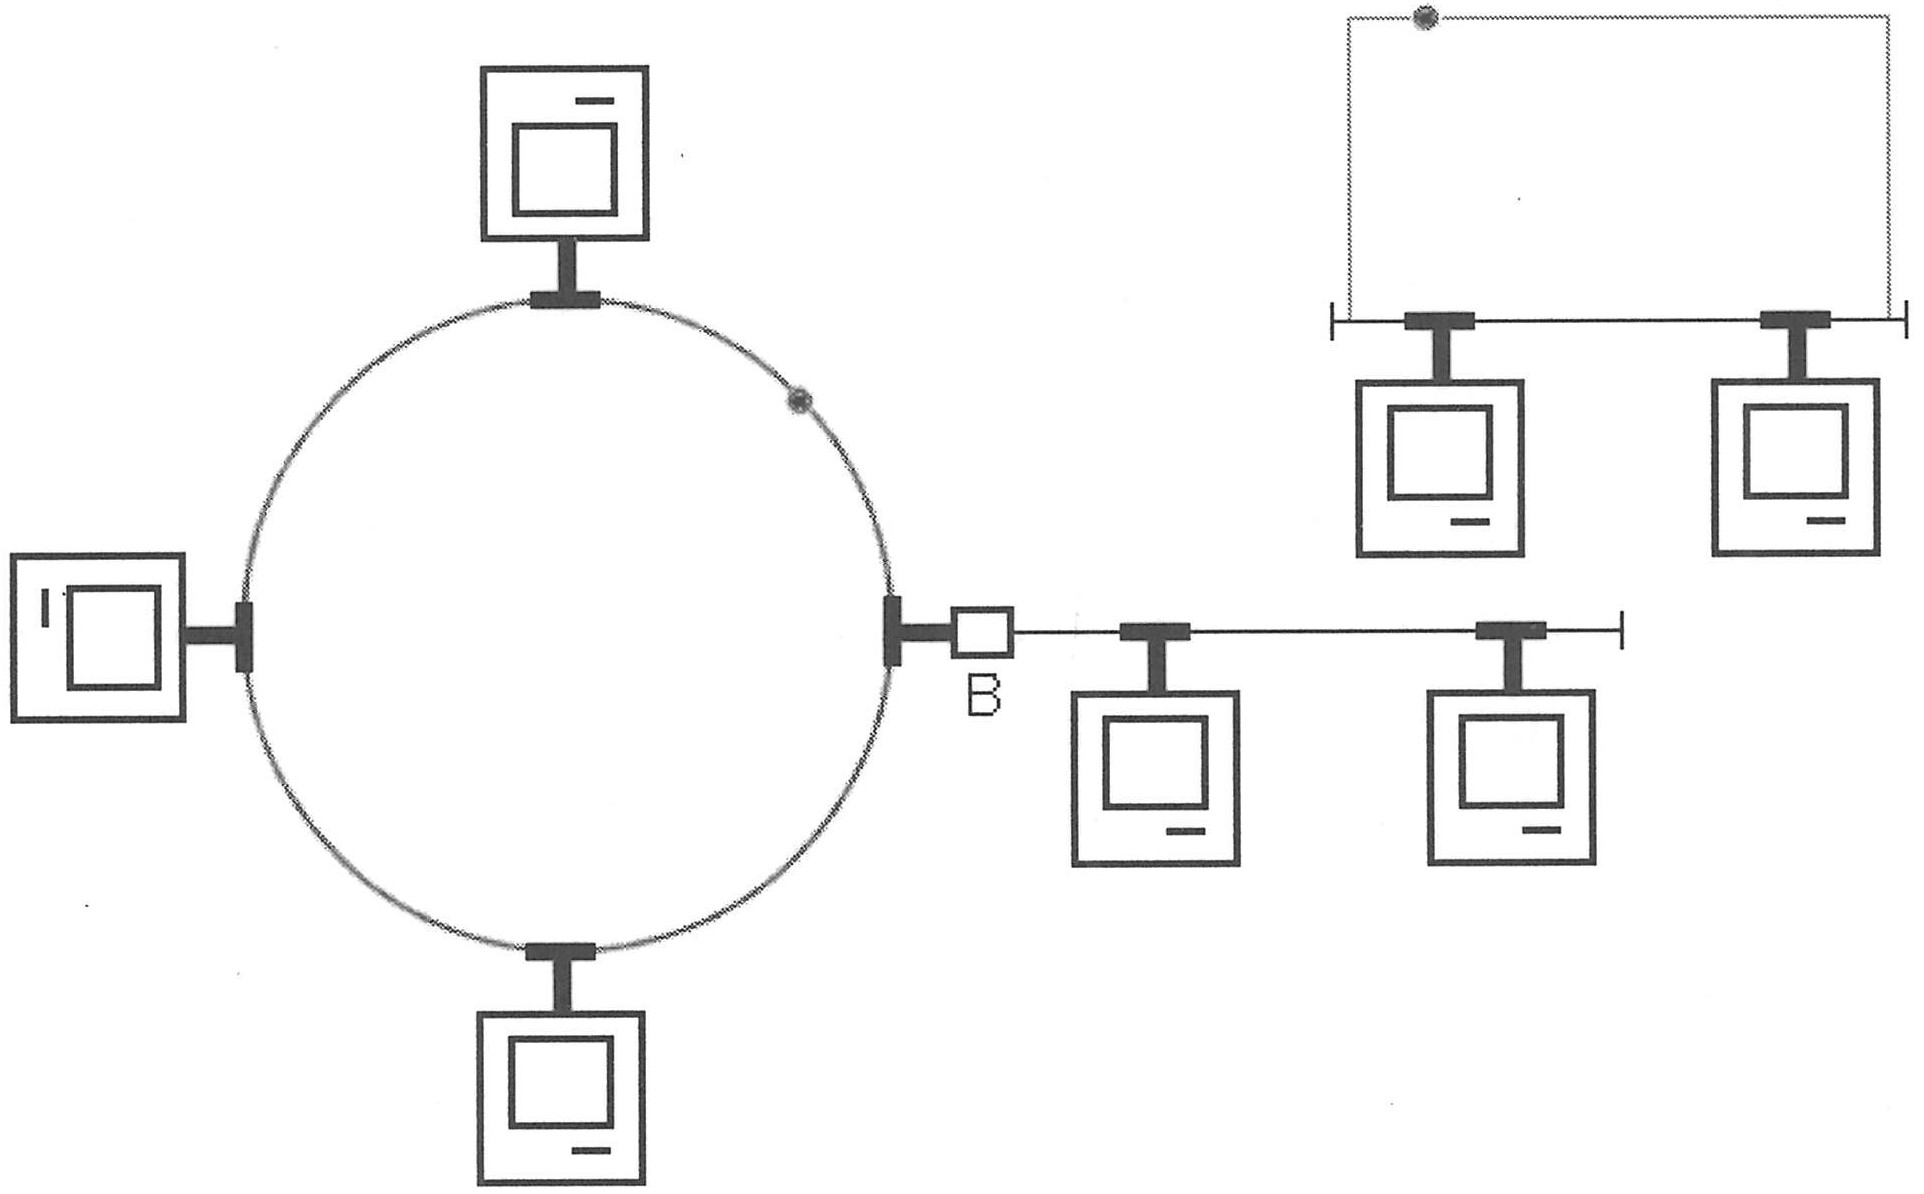
\includegraphics[width=\textwidth]{images/Token.jpg}
    \caption{Links: Token Ring. Rechts oben kleines Bild: Token wird auf einem Bus weitergereicht und am Ende wird es zum Anfang zurückgereicht und wieder gesendet.\cite{Schreiner2019}}
    \end{center}
\end{figure}

\subsection*{Was ist der Unterschied zwischen CSMA/CD und CSMA/CA? Wo werden sie verwendet?)}\label{sub:csma}\index{CSMA - Carrier Sense Multiple Access}
\textbf{CSMA: Carrier Sense Multiple Access}
\begin{itemize}
    \item Sender hört den Datenverkehr auf der Leitung ab (= carrier sense)
    \item Sender wartet, bis der Kanal frei ist
    \item sobald der Kanal frei ist, darf gesendet werden
    \item falls mehrere Sender (fast) gleichzeitig anfangen zu senden:\\Kollision $\rightarrow$ Wiederholung nach zufälliger Zeitspanne
\end{itemize}\,\\

\textbf{CSMA/CA (CA = Collision Avoidance)}
\begin{itemize}
    \item Kollisionsvermeidung durch zufällige Wartezeit nach Erkennung eines freien Kanals
    \item z.B. WLAN 802.11-DCF (Distributed Coordination Function)
\end{itemize}\,\\

\textbf{CSMA/CD (Collision Detection)}
\begin{itemize}
    \item sobald eine Kollision erkannt wird, wird die Übertragung abgebrochen
    \item z.B. Ethernet
\end{itemize}\,\\

\begin{tabularx}{\textwidth}{X|X}
    \multicolumn{1}{X}{CSMA/CD}&\multicolumn{1}{X}{CSMA/CA}\\
    \hline
    $\bullet$ Greift nach der Kollision&$\bullet$ Greift vor der Kollision\\
    $\bullet$ Genutzt in kabelgebundenen Netzwerken&$\bullet$ Genutzt in kabellosen Netzwerken\\
    $\bullet$ Reduziert die "'recovery time"' nach einer Kollision&$\bullet$ Minimiert Kollisionsgefahr\\
    $\bullet$ Bei Konflikt wird erneut gesendet&$\bullet$ Sendet zuerst die Info, dass etwas übermittelt wird\\
    $\bullet$ Effektiver als das einfache CSMA&$\bullet$ ähnlich effizient wie CSMA\\
\end{tabularx}

\subsection*{Was bedeutet "`Late Collision"'?}\index{Late Collision}
\begin{itemize}
    \item Definition:
    \begin{itemize}
        \item Late Collisions sind ein spezieller Typ von Kollisionen im Ethernet
        \item Kollision tritt nach den ersten 64 Bytes (512 bits) eines Frames auf (Mindestgrösse)
    \end{itemize}
    \item Ursachen:
    \begin{itemize}
        \item Ein wesentlich zu langes Netzwerkkabel
        \item Falsche Duplex-Einstellungen an Netzwerkkarte oder Switch
    \end{itemize}
\end{itemize}

\subsection*{Was muss man noch unbedingt über die physikalische Schicht und Zugriffsverfahren wissen?}
\begin{itemize}
    \item Übertragung nicht nur "`physisch"' per Kabel
    \begin{itemize}
        \item Schall
        \item Licht
        \item elektromagnetische Wellen
    \end{itemize}
    \item Geräte
    \begin{itemize}
        \item Hub
        \item Repeater
        \item Kabel
        \item Antennen
    \end{itemize}
\end{itemize}

\section{Antworten T2}
\subsection*{Was für Topologien findet man in Computernetzwerken?}\index{Netzwerk!Topologie}
Topologien beschreiben, wie Geräte in einem Netzwerk miteinander kommunizieren. Verschiedene Topologien haben Vor- und Nachteile betreffend Kommunikationsfluss, Ausfallsicherheit (Single Point of Failure) und in ihrer Komplexität (Routing oder physisch). Je nach Art können Topologien kombiniert werden.

\paragraph*{Gängigste Topologie-Typen}
\begin{itemize}
    \item Bus
    \begin{itemize}
        \item Vorteile
        \begin{itemize}
            \item geringe Kosten
            \item einfache Verkabelung
            \item keine aktiven Netzwerkkomponenten
        \end{itemize}
        \item Nachteile
        \begin{itemize}
            \item leicht abhörbar
            \item kann bei einer Störung leicht blockiert werden
            \item viele Kollisionen
        \end{itemize}
    \end{itemize}
    \item Ring
    \begin{itemize}
        \item Vorteile
        \begin{itemize}
            \item keine Kollisionen
            \item alle Stationen sind Verstärker
            \item gut skalierbar
        \end{itemize}
        \item Nachteile
        \begin{itemize}
            \item hohe Latenzen zu entfernten Knoten
            \item leicht abhörbar
            \item langsamere Datenübertragung
            \item hoher Energieaufwand
        \end{itemize}
    \end{itemize}
    \item Stern
    \begin{itemize}
        \item Vorteile
        \begin{itemize}
            \item leicht erweiterbar
            \item hoher Datendurchsatz
            \item Ausfall der Endpunkte hat keinen Einfluss auf das Netz
        \end{itemize}
        \item Nachteile
        \begin{itemize}
            \item Single Point of Failure beim Verteiler
        \end{itemize}
        \item Anwendung: Heimnetzwerke
    \end{itemize}
    \item Vermaschtes Netz
    \begin{itemize}
        \item Vorteile
        \begin{itemize}
            \item grundsätzlich sehr ausfallsicher
            \item hoher Datendurchsatz
        \end{itemize}
        \item Nachteile
        \begin{itemize}
            \item hoher Realisierungsaufwand
        \end{itemize}
        \item Anwendung: WAN
    \end{itemize}
\end{itemize}

\def\faktor{.4}
\def\rootfarbe{green!20!cyan!50!black}
\def\ballfarbe{green!50!cyan!75!black}

\tikzset{
    net root node/.style = {net node, minimum width=3*\faktor cm, ball color=\rootfarbe},
    net node/.style = {circle, minimum width=2*\faktor cm, inner sep=0pt, outer sep=0pt, ball color=\ballfarbe},
    net connect/.style = {line width=1pt, draw=black},
    net thick connect/.style = {net connect, line width=2.5pt},
}

\begin{multicols}{2}
\begin{figure}[H]
    \begin{center}
    \label{pic:TopologyLine}
    \begin{tikzpicture}
    \foreach \i in {0,2,4,6}
    \path (\i,0) node (n\i) [net node] {};
    \path [net connect] (n0) -- (n2) -- (n4) -- (n6);
    % \foreach \i in {0,2,4,6}
    % \path [net connect] (\i+2,0) -- (\i,0) node [net node] {};
    % \path node at (8,0) [net node] {};
    \end{tikzpicture}
    \caption{Linie}
    \end{center}
\end{figure}

\begin{figure}[H]
    \begin{center}
    \label{pic:TopologyBus}
    \begin{tikzpicture}
    \path [net thick connect]
        (0,0) -- (6,0);
    \foreach \i/\j in {2/-1,4/-1,1/1,3/1,5/1}
    \path [net connect] (\i,0) -- (\i,\j) node [net node] {};
    \end{tikzpicture}
    \caption{Bus Netz}
    \end{center}
\end{figure}

\begin{figure}[H]
    \begin{center}
        \label{pic:TopologyStar}
        \begin{tikzpicture}
        \node (root) [net root node] {};
        \foreach \i in {0,...,5}
            \path [net connect] (root) -- (-90+\i*60:2) node [net node] {};
        \end{tikzpicture}
        \caption{Stern Netz}
    \end{center}
\end{figure}

\columnbreak
\begin{figure}[H]
    \begin{center}
        \label{pic:TopologyRing}
        \begin{tikzpicture}
            \foreach \i in {0,...,5}
            \path (-90+\i*60:2) node (n\i) [net node] {};
            \path [net connect] (n0) -- (n1) -- (n2) -- (n3) -- (n4) -- (n5) -- (n0);
        \end{tikzpicture}
        \caption{Ring Netz}
    \end{center}
  \end{figure}

  \begin{figure}[H]
    \begin{center}
        \label{pic:TopologyMesh}
        \begin{tikzpicture}
        \foreach \i in {0,...,5}
            \path (-90+\i*60:2) node (n\i) [net node] {};
        \foreach \i in {0,...,5}
            \foreach \j in {2,3}
            \path [net connect]
                (n\i) -- (n\j);;
        \end{tikzpicture}
        \caption{Vermaschtes Netz}
    \end{center}
\end{figure}

\begin{figure}[H]
    \begin{center}
        \label{pic:TopologyFullMesh}
        \begin{tikzpicture}
        \foreach \i in {0,...,5}
            \path (-90+\i*60:2) node (n\i) [net node] {};
        \foreach \i in {0,...,5}
            \foreach \j in {0,...,5}
            \path [net connect]
                (n\i) -- (n\j);;
        \end{tikzpicture}
        \caption{Vollvermaschtes Netz}
    \end{center}
\end{figure}
\end{multicols}
\begin{figure}[H]
    \begin{center}
    \label{pic:TopologyTree}
    \begin{forest}
      for tree={
        edge=net connect,
        if level=0{%
          net root node,
          before typesetting nodes={
            repeat=2{
              append={[,
                net node,
                repeat=3{
                  append={[, net node]},
                },
              ]},
            },
          },
        }{},
      }
      []
    \end{forest}
    \caption{Baum Netz}
    \end{center}
\end{figure}

\subsection*{Wo ist der Unterschied zwischen \flqq{}Bandwidth\frqq, \flqq{}Throughput\frqq{} und \flqq{}Goodput\frqq? Wie kann man diese Konzepte visualisieren und verstehen?}\index{Bandbreite}\index{Bandwith}\index{Throughput}\index{Goodput}
\begin{itemize}
    \item \textbf{Bandwith (Bandbreite):} Gibt an, wie viel Daten \textbf{theoretisch} zu einem bestimmten Zeitpunkt von einer Quelle übertragen werdne könnten.
    \item \textbf{Throughput (Durchsatz):} Gibt an, wie viel Daten \textbf{effektiv} zu einem bestimmten Zeitpunkt von einer Quelle übertragen wurden.
    \item \textbf{Goodput (Datenduchsatz):} Gibt die \textbf{Netto-Datenmenge} (ohne Overhead) pro Zeit an, welche von einer Quelle übertragen werden.
\end{itemize}

\subsection*{Was ist \flqq{}Latency\frqq{} und \flqq{}Jitter\frqq? Wie kann man diese Konzepte visualisieren und verstehen?}
Die Latenz ist die Zeitverzögerung in einem Netzwerk zwischen der Anfrage und der Antwort. Beispielsweise die Zeit, bei dem mein Rechner die Antwort einer DNS-Anfrage bekommt.\\
Jitter ist die Zeitverzögerung zwischen einzelnen Anfragen.

\subsection*{Was muss man noch unbedingt über Topologien und "`Bandwidth"' wissen?}
//TODO

\section{Antworten T3}
\subsection*{Was sind die wichtigsten Merkmale von Kupferkabeln?}
//TODO
\subsection*{Was für Kupferkabelarten werden heutzutage in Computernetzwerken am häufigsten verwendet?}
//TODO
\subsubsection*{Wie sind sie aufgebaut?}
//TODO
\subsubsection*{Wie sehen die Stecker aus?}
//TODO
\subsection*{Worauf muss bei der Handhabung und Verlegung der Kupferkabel besonders geachtet werden und warum?}
//TODO
\subsection*{Woraus resultieren die Längenbeschränkungen der Kupferverkabelung?}
//TODO
\subsection*{Was muss man noch unbedingt über Kupferkabel wissen?}
//TODO

\section{Antworten T4}
\subsection*{Was sind die wichtigsten Merkmale von Glasfaserkabeln?}
//TODO
\subsubsection*{Wie sind sie aufgebaut?}
//TODO
\subsubsection*{Wie sehen die Stecker aus?}
//TODO
\subsection*{Worauf muss bei der Handhabung und Verlegung von Glasfaserkabeln besonders geachtet werden und warum?}
//TODO
\subsection*{Woraus resultieren die Längenbeschränkungen der Glasfaserkabelverkabelung?}
//TODO
\subsection*{Wo ist der Unterschied zwischen Multi- und Singlemode (Monomode)- Glasfasern?}
//TODO
\subsection*{Was sind die Vor- und Nachteile von Glasfaserkabel (im Vergleich zu Kupferkabeln)?}
//TODO
\subsection*{Was muss man noch unbedingt über Glasfaserkabel wissen?}
//TODO

\section{Antworten T5}
\subsection*{Was sind die wichtigsten Merkmale von \flqq{}Wireless Media\frqq?}\index{Wireless!Media}
Wireless beruht auf verschiedene Kommunikationstechnologien, welche kabellose Datenübertragung ermöglichen, anstatt auf kabelgebundene Technologien zurückzugreifen. Das Übertragungsmedium sind also Funkwellen.

\subsection*{Welche Wireless Access Geräte arbeiten auf Layer I?}\index{Wireless!Geräte}
Wireless Hubs \& Repeater.

\subsection*{Was für Wireless Standards gibt's in Computernetzwerken?}\index{Wireless!Standards}
\begin{table}[H]
    \resizebox{\textwidth}{!}{
    \begin{tabular}{|c|c|c|c|}
        \hline
        WLAN-Generation&WiFi 4&WiFi 5&WiFi 6 / 6E\\
        \hline
        IEEE-Standard&IEEE 802.11n&IEEE 802.11ac&IEEE 802.11ax\\
        \hline
        \makecell{Max.\\Übertragungsrate}&600 MBit/s&6'936 MBit/s&9'608 MBit/s\\
        \hline
        Max. Reichweite&100 m&50 m&50 m\\
        \hline
        Frequenzbereich&2,4 + 5 GHz&5 GHz&2,4 + 5 + 6 GHz\\
        \hline
        Max. Kanalbreite&40 MHz&160 MHz&160 MHz\\
        \hline
        Anwendungsbereiche&\makecell{Haushalte und\\wenige Firmen}&\makecell{Wenige Haushalte\\und viele Firmen}&\makecell{Bald neuer Standard\\für Haushalte und Firmen}\\
        \hline
    \end{tabular}}
\label{tab:WirelessStandards}
\caption{Wireless Standards und Merkmale}
\end{table}

\subsubsection*{Was sind ihre Hauptmerkmale und Anwendungsbereiche?}
Siehe vorherige Tabelle \ref{tab:WirelessStandards} unter \underline{\nameref{tab:WirelessStandards}}.

\subsection*{Was sind die Vor- und Nachteile von \flqq{}Wireless Access\frqq{} Methoden im Vergleich mit \flqq{}Wired Access\frqq?}
\begin{itemize}
    \item Vorteile
    \begin{itemize}
        \item Schnelle Erweiterung von Netzen
        \begin{itemize}
            \item Es müssen keine Kabel gezogen werden.
        \end{itemize}
        \item Kurzfristige Skalierung von Usern
        \begin{itemize}
            \item Neue Mitarbeiter können schnell und einfach ins Netz. Kostengünstiger und kein "`Kabelsalat"'.
        \end{itemize}
        \item Flexibilität / Mobilität
        \begin{itemize}
            \item Hotspots \& temporäre Netze
        \end{itemize}
    \end{itemize}
    \item Nachteile
    \begin{itemize}
        \item Übertragungsgeschwindigkeit
        \begin{itemize}
            \item Viele User teilen sich die verfügbare Bandbreite.
        \end{itemize}
        \item Umwelteinflüsse
        \begin{itemize}
            \item Funkstörungen durch andere Geräte
            \item Bauliche Gegebenheiten
        \end{itemize}
        \item Nettobandbreite
        \begin{itemize}
            \item Theoretische und praktische Geschwindigkeiten liegen teils weit auseinander.
        \end{itemize}
        \item Security
        \begin{itemize}
            \item Einfacher angreifbar, da kein physischer Zutritt in Gebäude nötig.
        \end{itemize}
    \end{itemize}
\end{itemize}
\part{SW 04 - Data Link Layer - Sicherungsschicht}
\section{Lernziele (Leitfragen)}
\begin{itemize}
    \item Was ist der Unterschied zwischen CSMA/CD und CSMA/CA? Wo werden sie verwendet?
    \item Was ist der Zweck der Sicherungsschicht?
    \item Wie ist die Sicherungsschicht aufgeteilt? Was ist die Hauptaufgabe der LLC und MAC Schichten?
    \item Welches sind die am häufigsten verwendeten Zugriffsverfahren?
    \item Was für Felder findet man in der Sicherungsschicht Frame?
    \item Was sind die wichtigsten Merkmale von MAC Adressen?
    \item Was machen Endgeräte, wenn ihre NIC ein Frame im Medium erkennen?
    \item Wie werden Sicherungsschicht Frames in einem Switch bearbeitet?
    \item Wie funktioniert der «Learn-and-forward» Prozess?
    \item Was ist der Unterschied zwischen «Unicast» und «Broadcast» Frames?
    \item Was ist der Zweck ARPs?
    \item Wie funktioniert ARP?
\end{itemize}

\section{Antworten}
\subsection*{Was ist der Unterschied zwischen CSMA/CD und CSMA/CA? Wo werden sie verwendet?}
\subsection*{Was ist der Zweck der Sicherungsschicht?}
\subsection*{Wie ist die Sicherungsschicht aufgeteilt? Was ist die Hauptaufgabe der LLC und MAC Schichten?}
Logical Link Control
\subsection*{Welches sind die am häufigsten verwendeten Zugriffsverfahren?}
\subsection*{Was für Felder findet man in der Sicherungsschicht Frame?}
\begin{itemize}
    \item Head
    \item Data
    \item Trailer
\end{itemize}
//TODO Frame Fields picture
\subsection*{Was sind die wichtigsten Merkmale von MAC Adressen?}
\begin{itemize}
    \item 48 bits = 12 hex-Ziffern = 6 bytes
    \item einzigartig
    \item Erste Hälfte von Hersteller, zweite Hälfte zufällig
\end{itemize}
\subsection*{Was machen Endgeräte, wenn ihre NIC ein Frame im Medium erkennen?}
\subsection*{Wie werden Sicherungsschicht Frames in einem Switch bearbeitet? }

\subsection*{Wie funktioniert der «Learn-and-forward» Prozess?}
\subsection*{Was ist der Unterschied zwischen «Unicast» und «Broadcast» Frames?}
\subsection*{Was ist der Zweck ARPs?}
Das Address Resolution Protocol vermittelt zwischen der Sicherungsschicht und der Netzwerkschicht.
\subsection*{Wie funktioniert ARP?}

\part{SW 05/06 - Network Layer - Vermittlungsschicht}\label{part:sw0506}
\section{Lernziele (Leitfragen) SW 05}
\begin{itemize}
    \item Was ist der Zweck der Vermittlungsschicht?
    \item Was für Protokolle findet man in der Vermittlungsschicht?
    \item Was sind die wichtigsten Merkmale des IPv4 Protokolls?
    \item Wie lange sind IPv4 Adressen?
    \item Wie sind IPv4 Adressen unterteilt?
    \item Wie findet man die Netzwerkadresse anhand der Hostadresse und der Subnetzmaske?
    \item Was ist die Verbindung zwischen Subnetzmasken und \flqq Slash Notation\frqq{}?
    \item Was ist der Unterschied zwischen Private und Public IPv4 Adressen?
    \item Wie werden Private IPv4 Adressen verwendet im Internet?
    \item Wieso brauchen wir Private IPv4 Adressen?
    \item Was ist eine Loopbackadresse? Wie wird diese Adresse verwendet?
    \item Was sind \flqq Link-Local\frqq{} (APIPA) Adressen? Wie und wann werden diese Adressen verwendet?
    \item Wie routet ein Host seine eigenen IPv4 Pakete?
    \item Was ist die Rolle der Default Gateway in dem Routing Prozess?
\end{itemize}

\section{Antworten}
\subsection*{Was ist der Zweck der Vermittlungsschicht?}
\begin{itemize}
    \item \textbf{Adressierung von Endgeräten }
    \item Datenkapselung
    \begin{itemize}
        \item IP kapselt das Transport Layer Segment
        \item IP kann entweder ein \textbf{IPv4 oder IPv6} Paket verwenden ohne Einfluss auf das Layer 4 Segment zu haben
        \item IP Paket \textbf{wird von allen Layer 3 Geräten untersucht}, während es durch das Netzwerk übertragen wird
        \item Die IP Adressierung ändert sich vom Ursprung (source) bis zum Ziel (destination) nicht, mit Ausnahme wenn NAT verwendet wird (Siehe Glossar: \gls{nat})
    \end{itemize}
    \item \textbf{Routen}
    \item Entkapselung
\end{itemize}\,\\
Siehe auch \underline{\hyperref[sub:SchichtenOSIModell]{Schichten des OSI Modells}} (Seite \pageref{sub:SchichtenOSIModell}).

\subsection*{Was für Protokolle findet man in der Vermittlungsschicht?}\index{IP - Internet Protocol}
Allgemein \textsl{Internet Protocol}. \textbf{IP - Internet Protocol (v4\&v6), IPsec - Internet Protocol Security, ICMP - Internet Control Message Protocol, IPX - Internet Packet Exchange (veraltet, von Firma Novell)}.

\subsection*{Was sind die wichtigsten Merkmale des IPv4 Protokolls?}\index{IP - Internet Protocol}
Die Funktionsweise vom Internet Protocol ist
\begin{itemize}
    \item Adressierung von Endgeräten
    \item Kapselung
    \item Routing
    \item Entkapselung
\end{itemize}

IP ist so gestaltet, dass es einen möglichst geringen "`Overhead"' hat. Folglich:
\begin{itemize}
    \item Es ist verbindungslos
    \begin{itemize}
        \item Keinen Verbindungsaufbau: Pakete werden einfach gesendet
        \item Keine Kontrollinformationen (synchronizations, acknowledgements, etc.)
        \item Das Ziel wird das Paket\dots\textbf{\textsl{vielleicht}}\dots erhalten
    \end{itemize}
    \item Es funktioniert nach dem \textsl{best effort} Prinzip
    \begin{itemize}
        \item Keine Garantie für Zustellung
        \item Kein Mechanismus um Daten erneut zu senden
        \item Unwissen darüber, ob Ziel betriebsbereit ist oder ob es das Paket erhalten hat
    \end{itemize}
    \item Unabhängig des Übertragungsmediums
    \begin{itemize}
        \item IP interessiert sich nicht über das Data Link Layer (Sicherungsschicht) oder des Physical Layer (physikalische Schicht)
        \item Mit einer Ausnahme: nicht die die maximale Übertragungseinheit, Maximum Transfer Unit (MTU), der Sicherungsschicht überschreiten!
        \begin{itemize}
            \item MTU muss durch das Data Link Layer gegeben werden
            \item Es ist unerwünscht, dass das Paket des Network Layers (Vermittlungsschicht) die MTU des Data Link Layer (Sicherungsschicht) überschreitet
            \item Was passiert, wenn das Paket grösser als die MTU ist? ($\rightarrow$ Fragmentierung des Paketes in mehrere Pakete)
        \end{itemize}
    \end{itemize}
\end{itemize}

\subsection*{Wie lange sind IPv4 Adressen?}
4 bytes = 32 bits

\subsection*{Wie sind IPv4 Adressen unterteilt?}
\begin{itemize}
    \item Netzwerkadresse
    \item Hostadresse
    \item Broadcast Adresse
\end{itemize}

\subsection*{Wie findet man die Netzwerkadresse anhand der Hostadresse und der Subnetzmaske?}
Angenommen, die Hostadresse ist 192.168.10.11 und die Subnetzmaske 255.255.248.0. Man stellt beide Adressen als Binärwerte dar. Die Bits der beiden Adressen werden UND-verknüpft ($1\wedge1=1,\, 0\wedge1=0$).\\

\begin{tabularx}{\textwidth}{lccccccc}
    % 1 & 2 & 3 & 4 & 5 & 6 & 7 & 8
    & \multicolumn{5}{c}{\cellcolor{lime}Netzwerk Teil}&&\cellcolor{violet!50}Host Teil\\
    \multirow{2}{*}{IPv4 Hostadresse}&\cellcolor{lime}192&\cellcolor{lime}.&\cellcolor{lime}168&\cellcolor{lime}.&\cellcolor{lime}\color{orange}10&.&\cellcolor{violet!50}11\\
    &1100 0000&.&1010 1000&.&0000 1010&.&0000 1011\\

    \multicolumn{8}{c}{}\\

    \multirow{2}{*}{Subnetzmaske}&255&.&255&.&248&.&\cellcolor{violet!50}0\\
    &\cellcolor{lime}1111 1111&\cellcolor{lime}.&\cellcolor{lime}1111 1111&\cellcolor{lime}.&\cellcolor{lime}1111 1\noindent\colorbox{violet!50}{000}&.&\cellcolor{violet!50}0000 0000\\

    \hline

    \multirow{2}{*}{IPv4 Netzwerkadresse}&192&.&168&.&8&.&0\\
    &1100 0000&.&1010 1000&.&0000 1000&.&0000 0000\\
\end{tabularx}
{\color{red}Achtung!} Die orange 10 gehört eigentlich schon zum Host. Das dritte Byte in der Subnetzmaske zeigt welche Bits zum Netzwerk gehören und welche zum Host. Die Netzwerkadresse ist 192.168.8.0/21, der Hostbereich also 192.168.8.1-192.168.15.254. Betrachtet man die 1000 bei der Subnetzmaske und diese dann auf 1111 "`auffüllt"', gibt das ja 15. Deswegen ist der Hostbereich auf diesem Byte 8-15.

\subsection*{Was ist die Verbindung zwischen Subnetzmasken und \flqq Slash Notation\frqq{}?}
Die Subnetzmaske stellt die 4 Bytes in dezimaler Form dar. Sie definiert, welcher Bereich zu welchem Netz gehört. Die Slash Notation gibt an, wie viele 1 von links nach rechts es gibt.

\subsection*{Was ist der Unterschied zwischen Private und Public IPv4 Adressen?}\label{sub:private_public_IP}
Auf private IPv4 Adressen kann von aussen nicht direkt zugegriffen werden. Diese sind nach aussen hin unsichtbar.

\subsection*{Wie werden Private IPv4 Adressen verwendet im Internet?}
Gar nicht. Mittels NAT wird die private Adresse in eine öffentliche getauscht. Jeder Router bekommt vom Internetprovider (z.B. Swisscom, UPC etc.) eine öffentliche Adresse zugewiesen. Öffentliche IP-Adressen sind einzigartig, private kommen aber in jedem LAN vor.

\subsection*{Wieso brauchen wir Private IPv4 Adressen?}
Um innerhalb des LANs auf Endgeräte zugreifen zu können. Auch deswegen, weil es inzwischen mehr Netzwerkgeräte gibt als es IP-Adressen zur Verfügung hat.

\subsection*{Was ist eine Loopbackadresse? Wie wird diese Adresse verwendet?}
Die Loopbackadresse zeigt auf den eigenen Host, das eigene NIC. Diese wird meistens dazu genutzt, um Programme, die als Server dienen können, lokal zu betreiben oder um zu überprüfen, ob die eigene Netzwerkkarte betriebsbereit ist.

\subsection*{Was sind \flqq Link-Local\frqq{} (APIPA) Adressen? Wie und wann werden diese Adressen verwendet?}\index{APIPA - \acrlong{apipa}}\label{sub:APIPA}
\acrfull{apipa} ist eine sogenannte Link-Local Address. Es ist eine vom Betriebssystem automatisch zugewiesene IP-Adresse, falls das System auf DHCP eingestellt ist, jedoch nichts vom DHCP offeriert wurde. Dies weil entweder kein DHCP-Server im Netzwerk vorhanden ist oder dieser keine Antwort gibt.\\Der Adressbereich in IPv4 ist 169.254.0.0/16 (169.254.0.0 - 169.254.255.255).

\subsection*{Wie routet ein Host seine eigenen IPv4 Pakete?}
Er schickt sie an den Gateway, vorausgesetzt es geht ins Internet. Im LAN geht es direkt an das Ziel.

\subsection*{Was ist die Rolle der Default Gateway in dem Routing Prozess?}
Geht ein Datenpaket ins Internet, "`übersetzt"' der Router die private IP-Adresse in eine öffentliche. (Siehe Glossar: \gls{nat})

\section{Lernziele (Leitfragen) SW 06}
\begin{itemize}
    \item How do I find out my IPv4 configuration?
    \item How do I find the IP address associated to a URL?
    \item How do I determine if a host is “up” given its IP or URL?
    \item How do I find out which intermediate network devices are there between my host and another host, given its IPv4 address (or URL)?
    \item Wieso brauchen wir IPv6? Was sind die Nachteile von IPv4?
    \item Wie lange sind IPv6 Adressen?
    \item Was sind die Regeln, um eine IPv6 Adresse zu komprimieren?
    \item Wie sind IPv6 Adressen unterteilt?
    \item Was für IPv6 unicast Adress Arten gibt es?
    \item Über welche IPv6 unicast Adressen sollte ein richtig konfigurierte Host mindestens verfügen?
    \item Wie sind IPv6 Global Unicast Addresses (GUAs) unterteilt?
    \item Welche Mechanismen werden verwendet, um IPv4 und IPv6 Netzwerken miteinander zu verbinden?
\end{itemize}

\section{Antworten}
\subsection*{How do I find out my IPv4 configuration?}
\begin{multicols}{2}
    Windows: \texttt{ipconfig [/all]}
    \begin{figure}[H]
        \begin{center}
        \label{pic:ipconfig}
        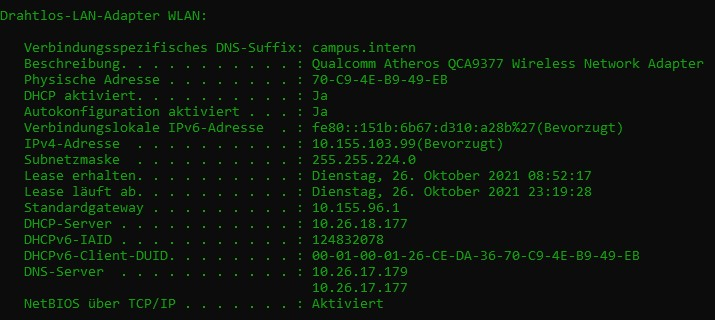
\includegraphics[width=.5\textwidth]{images/ipconfig.jpg}
        \caption{Adapterkonfiguration in Windows mit \texttt{ipconfig /all}}
        \end{center}
    \end{figure}
    \columnbreak
    Unix: \texttt{ifconfig}
    \begin{figure}[H]
        \begin{center}
        \label{pic:ifconfig}
        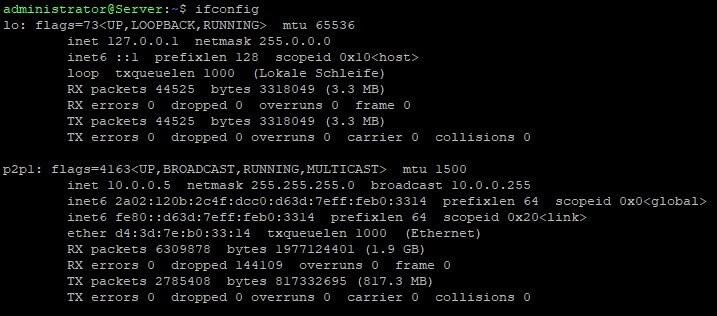
\includegraphics[width=.5\textwidth]{images/ifconfig.jpg}
        \caption{Adapterkonfiguration in Ubuntu mit \texttt{ifconfig}}
        \end{center}
    \end{figure}
\end{multicols}
\subsection*{How do I find the IP address associated to a URL?}
\begin{multicols}{2}
    \texttt{nslookup <URL>}
    \begin{figure}[H]
        \begin{center}
        \label{pic:nslookup_win{Sprungmarke}}
        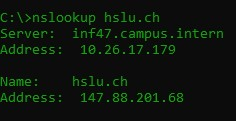
\includegraphics[width=.5\textwidth]{images/nslookup_win.jpg}
        \caption{\texttt{nslookup} in Windows}
        \end{center}
    \end{figure}
    \columnbreak
    \vfill\null
    \begin{figure}[H]
        \begin{center}
        \label{pic:nslookup_unix}
        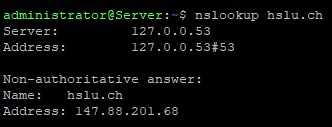
\includegraphics[width=.5\textwidth]{images/nslookup_unix.jpg}
        \caption{\texttt{nslookup} in Ubuntu}
        \end{center}
    \end{figure}
\end{multicols}
\pagebreak
\subsection*{How do I determine if a host is “up” given its IP or URL?}
\begin{multicols}{2}
    Windows:
    \begin{itemize}
        \item \texttt{ping [-4] <URL>}
        \item \texttt{ping <IPv4-Adresse>}
    \end{itemize}
    \begin{figure}[H]
        \begin{center}
        \label{pic:ping_win}
        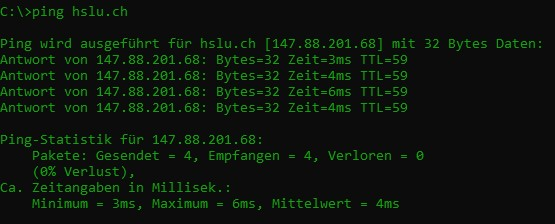
\includegraphics[width=.5\textwidth]{images/ping_win.jpg}
        \caption{\texttt{ping} in Windows}
        \end{center}
    \end{figure}
    \columnbreak
    Unix: \texttt{ping <IPv4-Adresse | URL>} (Ctrl+C zum abbrechen)
    \vfill\null
    \begin{figure}[H]
        \begin{center}
        \label{pic:ping_unix}
        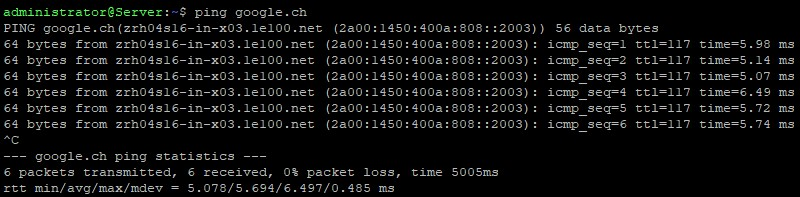
\includegraphics[width=.5\textwidth]{images/ping_unix.jpg}
        \caption{\texttt{ping} in Ubuntu}
        \end{center}
    \end{figure}
\end{multicols}
\subsection*{How do I find out which intermediate network devices are there between my host and another host, given its IPv4 address (or URL)?}
\begin{multicols}{2}
    Windows:
    \begin{itemize}
        \item \texttt{tracert [-4] <URL>}
        \item \texttt{tracert <IPv4 Address>}
    \end{itemize}
    \begin{figure}[H]
        \begin{center}
        \label{pic:tracert}
        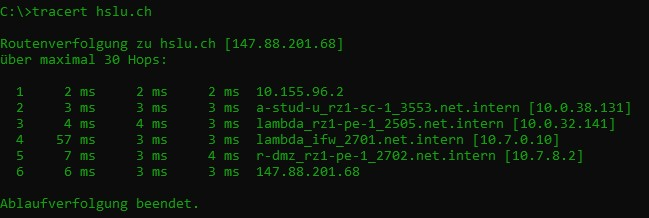
\includegraphics[width=.5\textwidth]{images/tracert.jpg}
        \caption{\texttt{tracert} in Windows}
        \end{center}
    \end{figure}
    %\vfill\null
    \columnbreak
    Unix: \texttt{traceroute <IPv4 Adress | URL>}
    \begin{figure}[H]
        \begin{center}
        \label{pic:traceroute}
        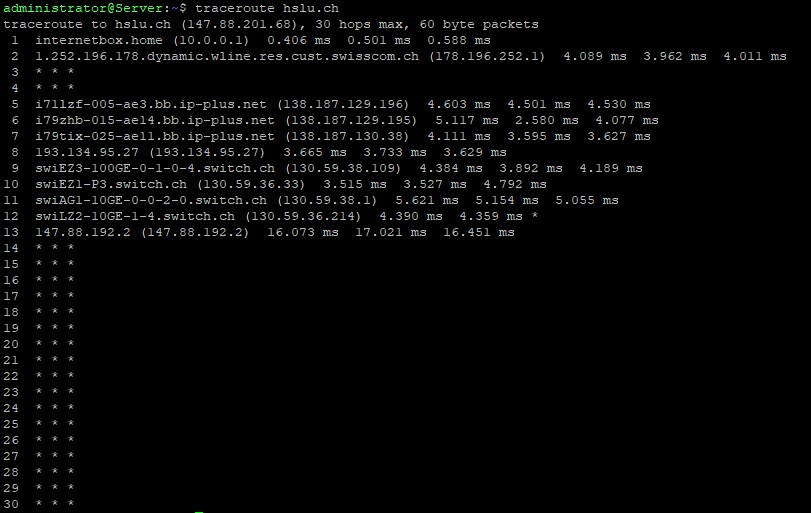
\includegraphics[width=.5\textwidth]{images/traceroute.jpg}
        \caption{\texttt{traceroute} in Ubuntu}
        \end{center}
    \end{figure}
\end{multicols}

\subsection*{Wieso brauchen wir IPv6? Was sind die Nachteile von IPv4?}
//TODO
\subsection*{Wie lange sind IPv6 Adressen?}
128 bit
\subsection*{Was sind die Regeln, um eine IPv6 Adresse zu komprimieren?}
//TODO
\subsection*{Wie sind IPv6 Adressen unterteilt?}
//TODO
\subsection*{Was für IPv6 unicast Adress Arten gibt es?}
//TODO
\subsection*{Über welche IPv6 unicast Adressen sollte ein richtig konfigurierte Host mindestens verfügen?}
\begin{itemize}
    \item 64 bit prefix
    \begin{itemize}
        \item \textbf{Global Routing Prefix}: Portion of the address that is assigned by the provider, such as an ISP, to a customer or site. The global routing prefix will vary depending on ISP policies.
        \item \textbf{Subnet ID}: Portion between the Global Routing Prefix and the Interface ID. The Subnet ID is used by an organization to identify subnets within its site.
    \end{itemize}
    \item Interface ID: Equivalent to the host portion of an IPv4 address.
\end{itemize}
\subsection*{Wie sind IPv6 Global Unicast Addresses (GUAs) unterteilt?}
//TODO
\subsection*{Welche Mechanismen werden verwendet, um IPv4 und IPv6 Netzwerken miteinander zu verbinden?}
\begin{enumerate}
    \item Dual stack - The devices run both IPv4 and IPv6 protocol stacks simultaneously.
    \item Tunneling - A method of transporting an IPv6 packet over an IPv4 network. The IPv6 packet is encapsulated inside an IPv4 packet.
    \item Translation - Network Address Translation 64 (NAT64) allows IPv6-enabled devices to communicate with IPv4-enabled devices using a translation technique similar to NAT for IPv4.
\end{enumerate}
\part{SW 07 - Transport Layer - Transportschicht}
\section{Lernziele (Leitfragen)}
\begin{itemize}
    \item Was ist der Zweck der Transportschicht?
    \item Was für Protokolle findet man in der Transportschicht?
    \item Was sind die wichtigsten Merkmale des TCP Protokolls?
    \item Was sind die wichtigsten Merkmale des UDP Protokolls?
    \item Wozu werden Ports in der Transportschicht verwendet?
    \item Was ist ein Socket?
    \item Was ist ein \flqq{}Socket Pair\frqq?
    \item Geben Sie Beispiele von Anwendungen die TCP verwenden
    \item Für welche Applikationsarten ist UDP besser geeignet als TCP?
    \item Welches Portintervall verwenden normalerweise bekannte Netzwerkapplikationen und -dienste?
    \item Wie realisiert TCP zuverlässige Verbindungen?
    \item Was ist der Zweck des TCP Handshake?
    \item Wie funktioniert der TCP Handshake?
    \item Wie werden Verbindungen in TCP richtig beendet?
    \item Was ist der Zweck von \flqq{}Selective Acknowledgements\frqq?
\end{itemize}

\section{Antworten}
\subsection*{Was ist der Zweck der Transportschicht?}
\begin{itemize}
    \item Multiplexing: Logische Kommunikation zwischen Applikationen, welche auf verschiedenen Hosts laufen
    \item Link zwischen Application Layer und darunterliegenden Layern
    \item Individuelle Kommunikationen verfolgen (jeder Tab im Browser) //TODO pic
    \item Segmentierung der Daten und wieder zusammenfügen
    \item Header Information hinzufügen
    \item Identifizieren, Teilen und verschiedene Konversationen managen
    \item Segmentierung //TODO Folie schauen
\end{itemize}
\subsection*{Was für Protokolle findet man in der Transportschicht?}
\begin{itemize}
    \item TCP - Transmission Control Protocoll
    \begin{itemize}
        \item Zuverlässigkeit - Reliability
        \begin{itemize}
            \item Nummerieren von Datensegmenten
            \item Bestätigen von übertragenen Daten
            \item Erneutes Senden von Daten, wenn Zeit abgelaufen
            \item Reorganisation von Daten, wenn in falscher Reihenfolge empfangen: $1,3,5,4,2 \rightarrow 1,2,3,4,5$
        \end{itemize}
        \item Durchsatzkontrolle - Flow Control
        \begin{itemize}
            \item Effizienteste Rate für Empfänger
        \end{itemize}
    \end{itemize}
    \item UDP - User Datagram Protocol
    \begin{itemize}
        \item //TODO
    \end{itemize}
\end{itemize}
\subsection*{Was sind die wichtigsten Merkmale des TCP Protokolls?}
//TODO
\subsection*{Was sind die wichtigsten Merkmale des UDP Protokolls?}
//TODO
\subsection*{Wozu werden Ports in der Transportschicht verwendet?}
//TODO
\subsection*{Was ist ein Socket?}
Ein Socket ist die Kombination von Source IP Address \& Source Port oder Destination IP Address \& Destination Port
\subsection*{Was ist ein \flqq{}Socket Pair\frqq?}
Unique Identifier für eine Verbindung.
\subsection*{Geben Sie Beispiele von Anwendungen die TCP verwenden}
\begin{itemize}
    \item Mail (POP, IMAP)
    \item Secure Shell (SSH)
    \item FTP
    \item HTTP
\end{itemize}
\subsection*{Für welche Applikationsarten ist UDP besser geeignet als TCP?}
\begin{itemize}
    \item DHCP
    \item DNS
    \item SNMP
    \item TFTP
    \item VoIP
    \item Video Conferencing
\end{itemize}
\subsection*{Welches Portintervall verwenden normalerweise bekannte Netzwerkapplikationen und -dienste?}
\begin{itemize}
    \item Low Ports / Well-known Ports: 0-1023, //TODO
    \item Registered Ports: 1024-49151, //TODO
    \item Private and/or Dynamic Ports: 49152-65535, //TODO
\end{itemize}
\subsection*{Wie realisiert TCP zuverlässige Verbindungen?}
//TODO
\subsection*{Was ist der Zweck des TCP Handshake?}
\begin{itemize}
    \item Wissen, dass Server da ist
    \item Client ist fähig Verbindung herzustellen
    \item Server weiss, dass Client verbinden möchte
    \item Vereinbarung zwischen Geräten über Session Control Parametern und optionalen Eigenschaften
\end{itemize}
\subsection*{Wie funktioniert der TCP Handshake?}
//TODO
\subsection*{Wie werden Verbindungen in TCP richtig beendet?}
//TODO
\subsection*{Was ist der Zweck von \flqq{}Selective Acknowledgements\frqq?}
//TODO
\end{document}